\chapter{Start-up and Shutdown Procedures}
\label{sec::B_su}
In this chapter, we will briefly document how to run the software that was developed within this thesis. In section \ref{sec::B1_rr}, we will introduce how the Heicub robot is supposed to be started, while in the subsequent section \ref{sec::B2_ss}, we will explain how to run the robot within the simulation environment Gazebo. Furthermore, once the robot has been started, either in real or in simulation, it is possible to use the provided pattern generator for control in real-time with the terminal interface or the Android joystick app. Both possibilities will be explained in section \ref{sec::B3_sp}. Finally, a short demonstration for the behavioral augmentation is given in section \ref{sec::B4_ba}.
\FloatBarrier
\section{Real Robot Start-up}
\label{sec::B1_rr}
\begin{enumerate}
	\item Turn on the icubsrv (figure \ref{fig::B1_icubsrv}), username is \inlinecode{bash}{icub}, ask someone at the ORB for the password.%password is \inlinecode{bash}{icub}.
	\begin{figure}[h!]
		\centering
		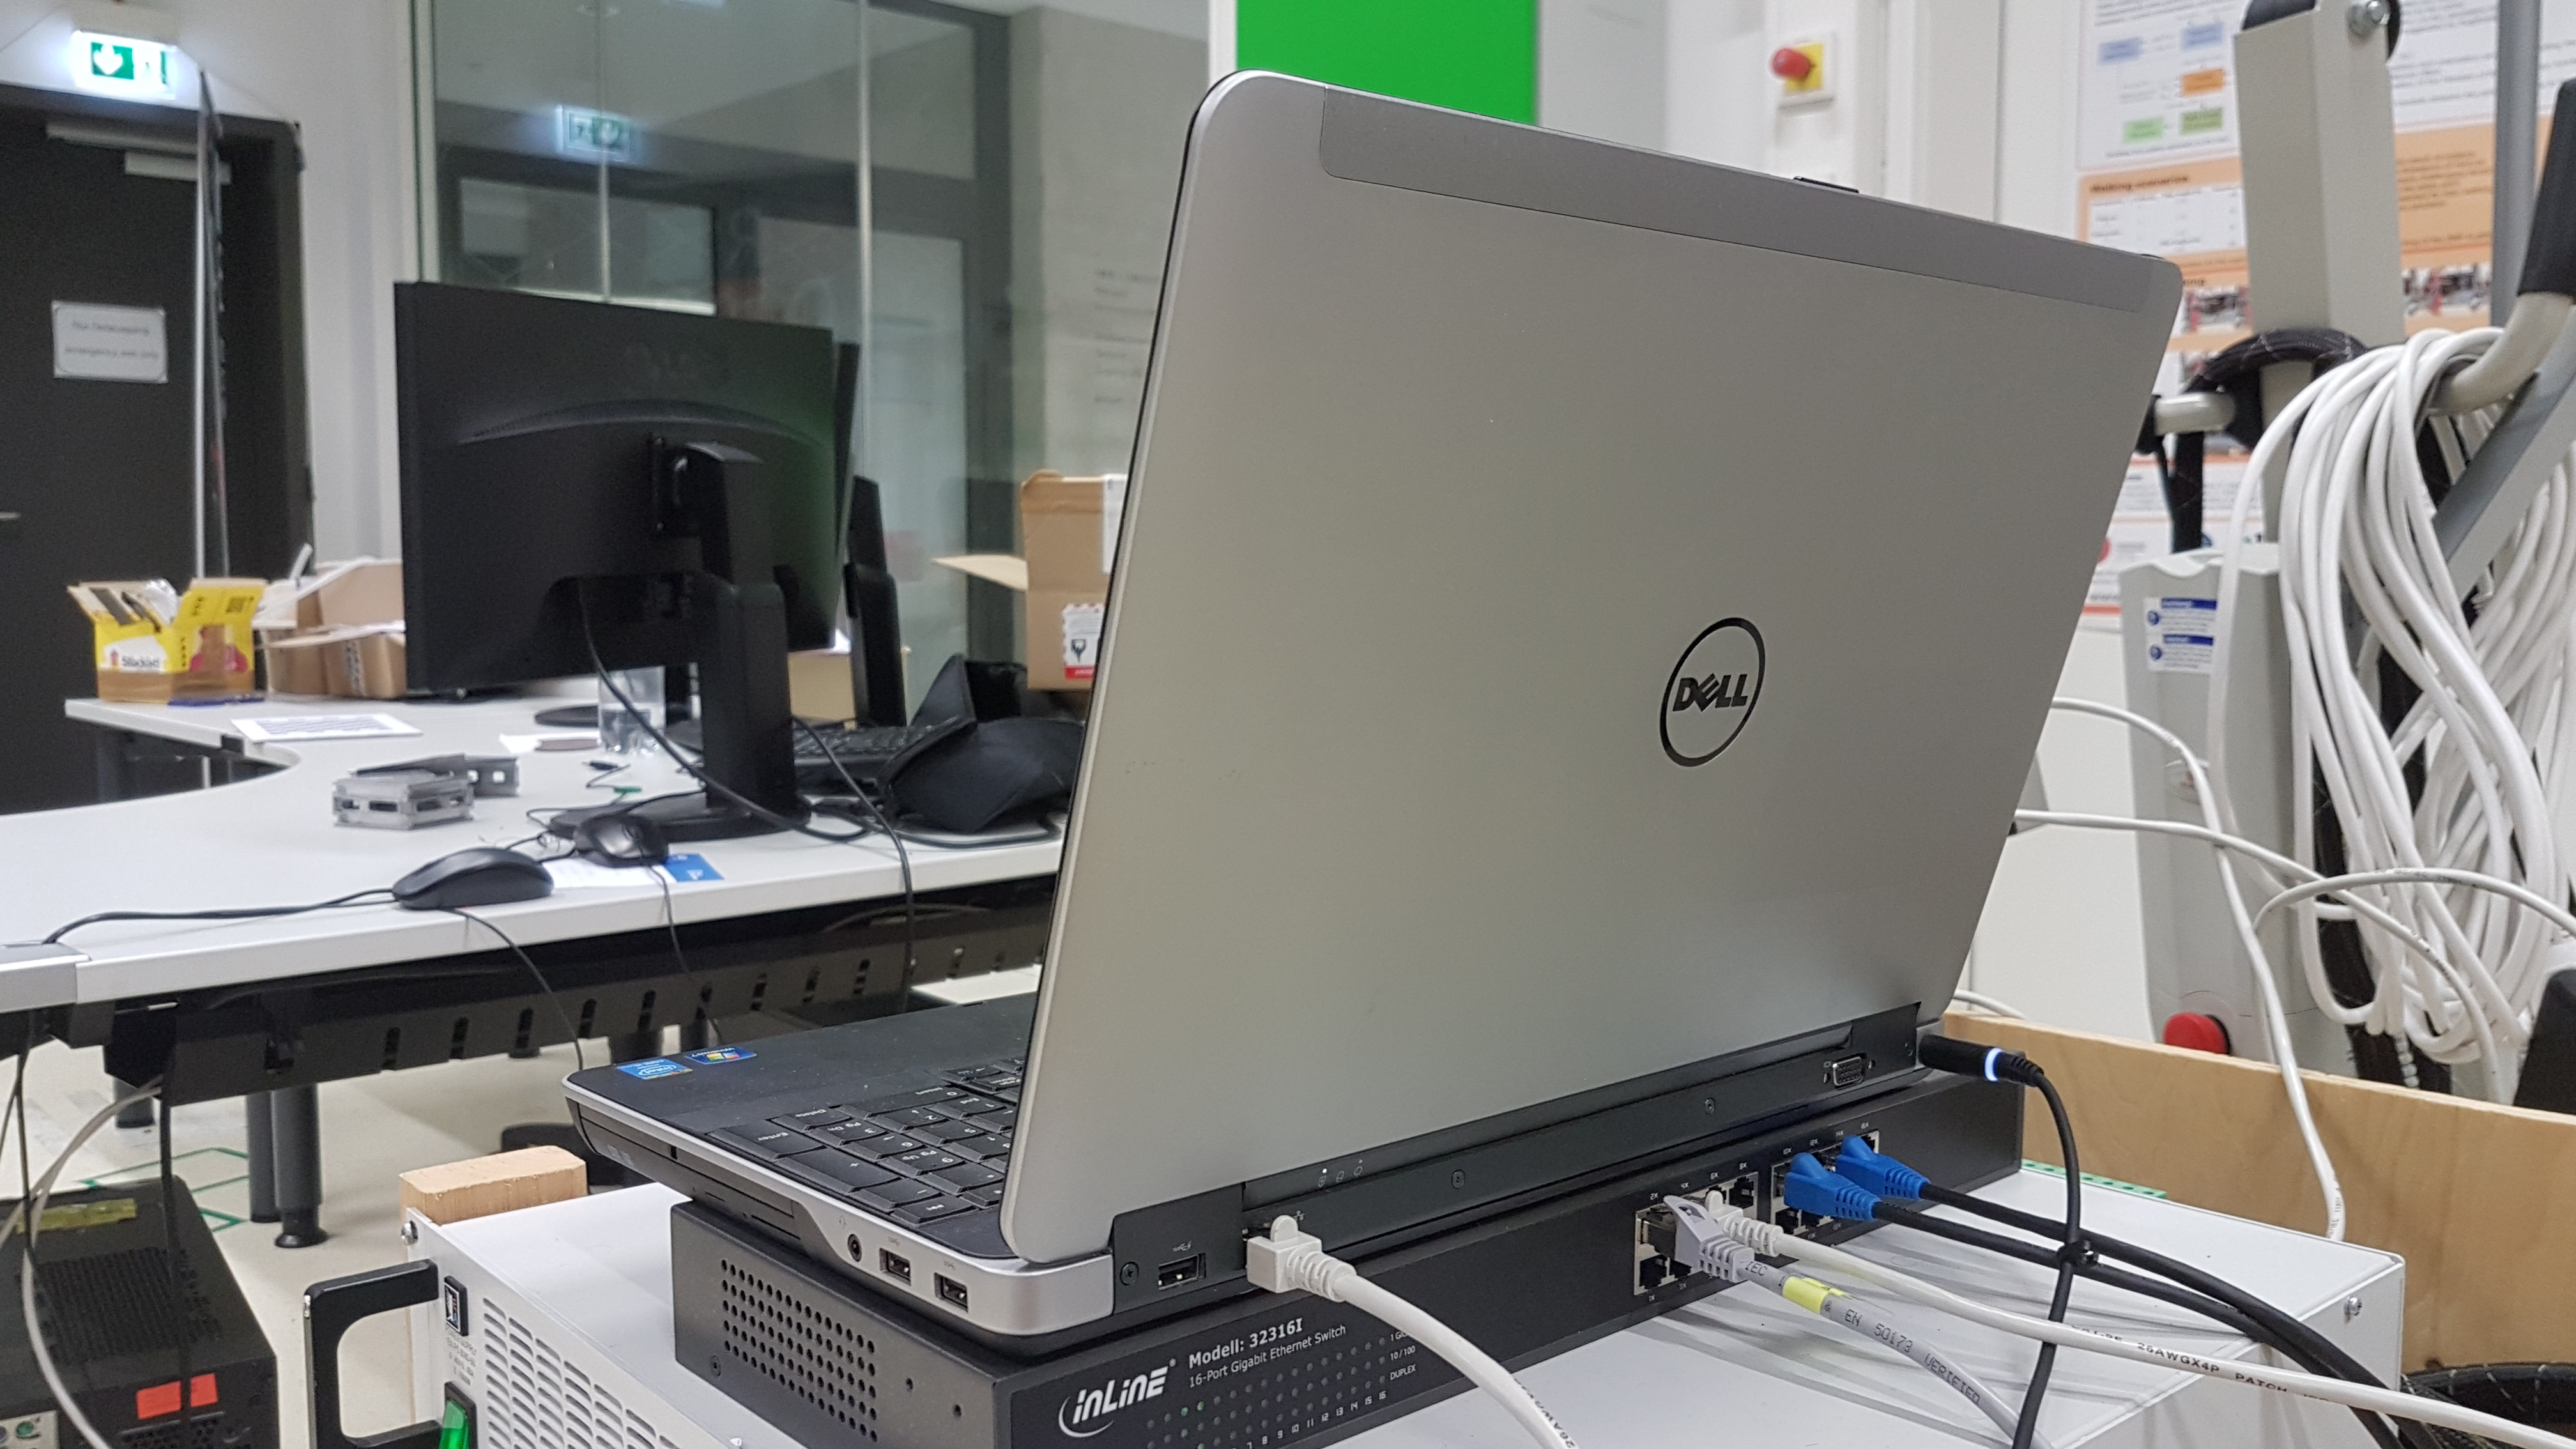
\includegraphics[scale=.04]{chapters/08_appendix/img/icubsrv.jpg}
		\caption{The icubsrv is the Dell laptop. Below it the switch.}
		\label{fig::B1_icubsrv}
	\end{figure}
	\item Turn on the power suppliers (figure \ref{fig::B1_ps}), and keep the red button pressed (figure \ref{fig::B1_red} (a)). The suppliers should initially provide 13V and 0V, if not, do no proceed.
	\begin{figure}[h!]
		\centering
		\subcaptionbox{Turn on these buttons.}%
		[.4\linewidth]{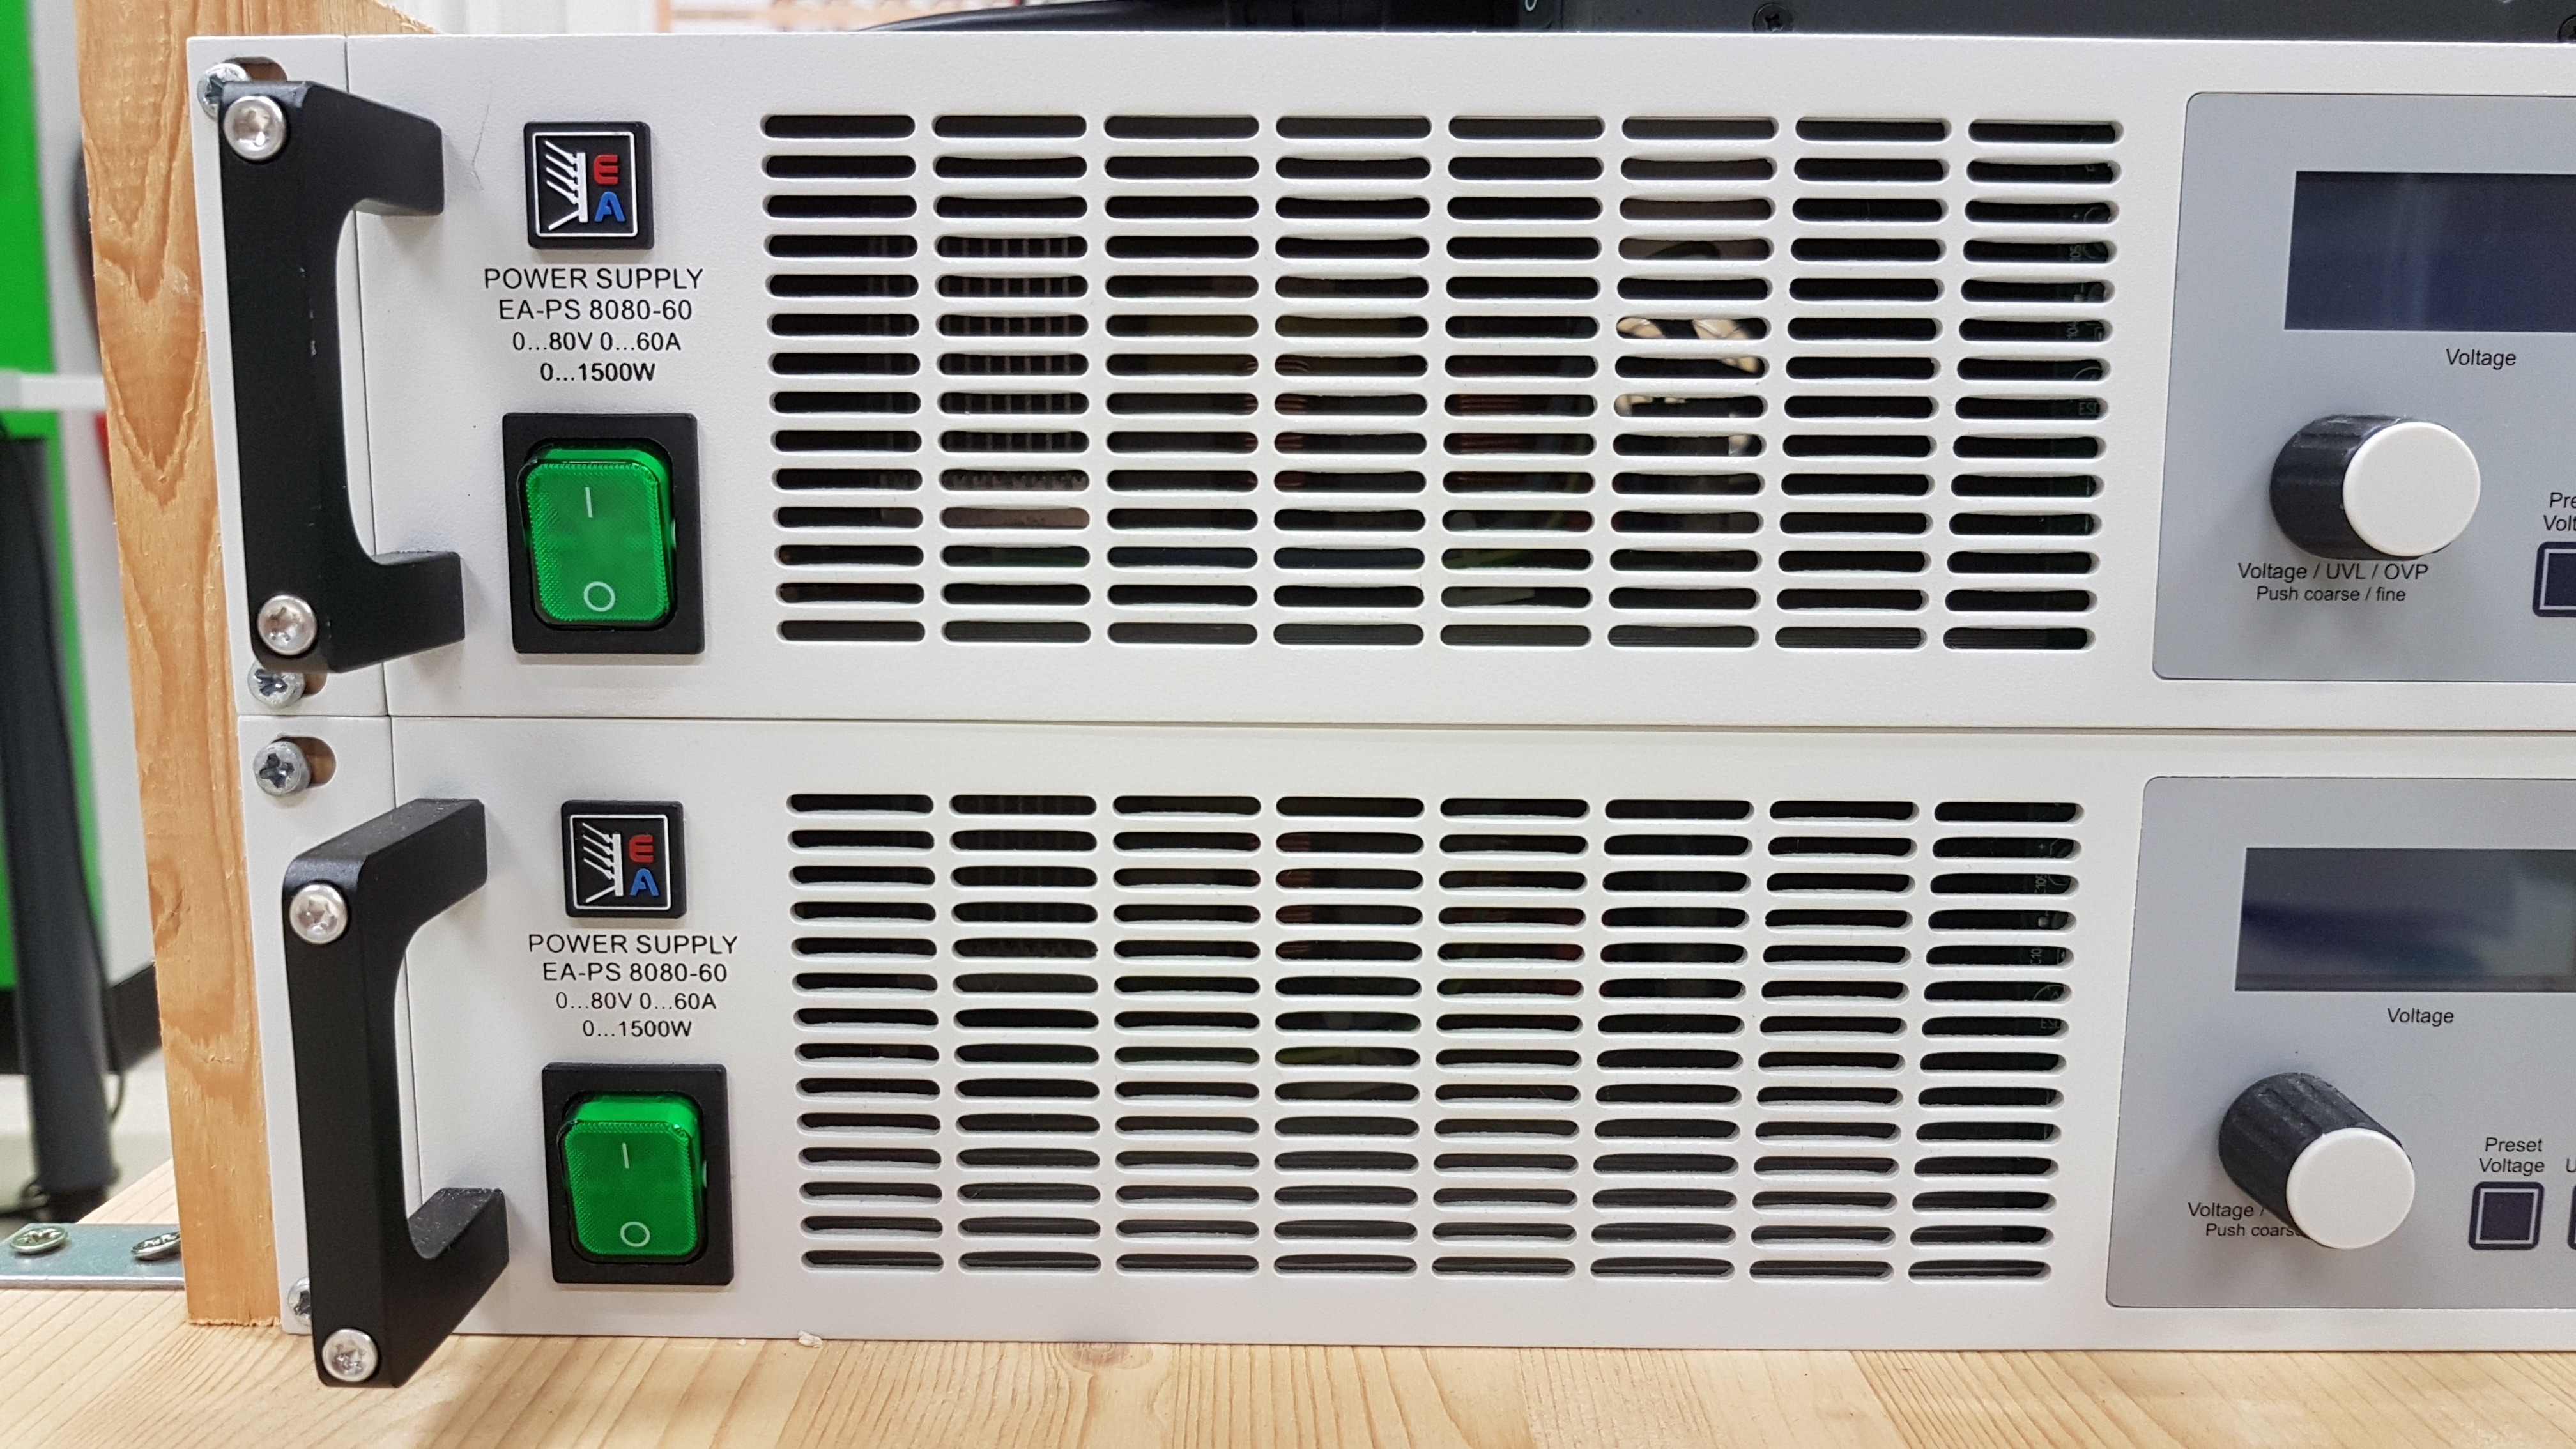
\includegraphics[scale=.04]{chapters/08_appendix/img/power_supply.jpg}}
		\subcaptionbox{Expected initial voltage.}%
		[.4\linewidth]{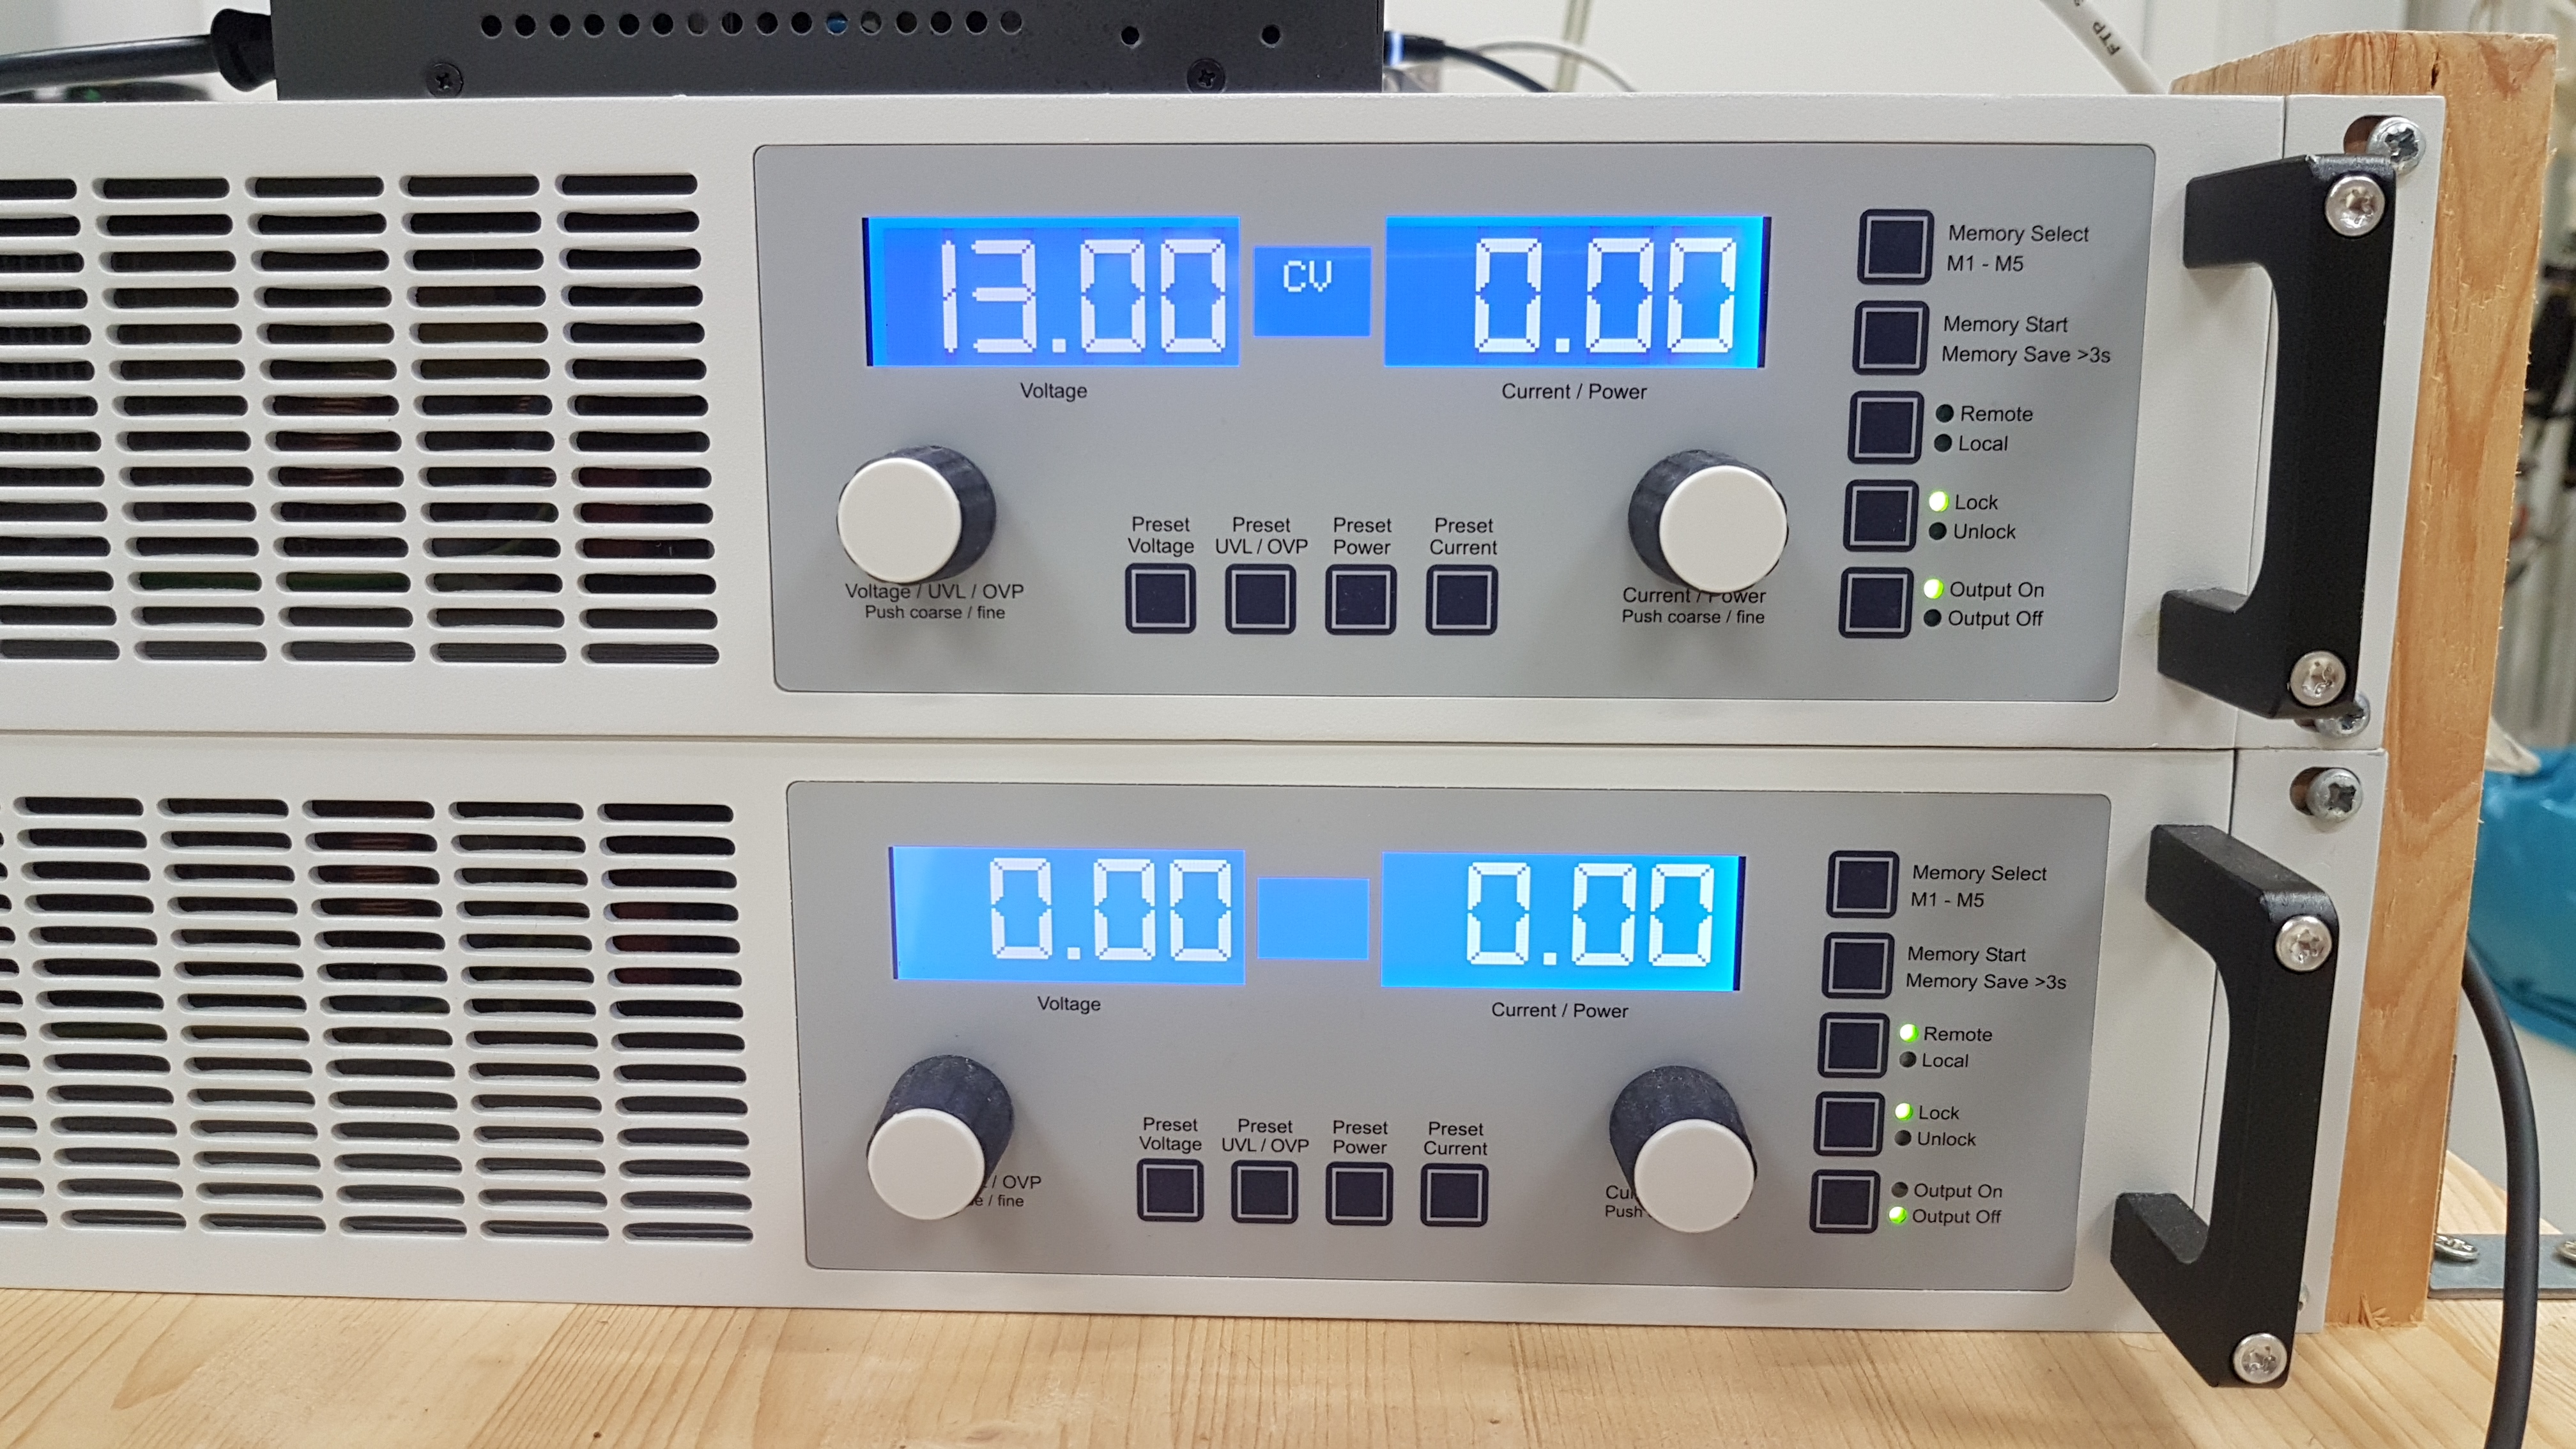
\includegraphics[scale=.04]{chapters/08_appendix/img/power_supply_13.jpg}}
		\caption{Power suppliers.}
		\label{fig::B1_ps}
	\end{figure}
	\item Turn on the pc104 (figure \ref{fig::B1_cpu_motor} (a)). At this step you may want to wait up to 5 minutes, to give the board computer enough time to start.
	\begin{figure}[h!]
		\centering
		\subcaptionbox{Turn on the CPU of pc104.}%
		[.4\linewidth]{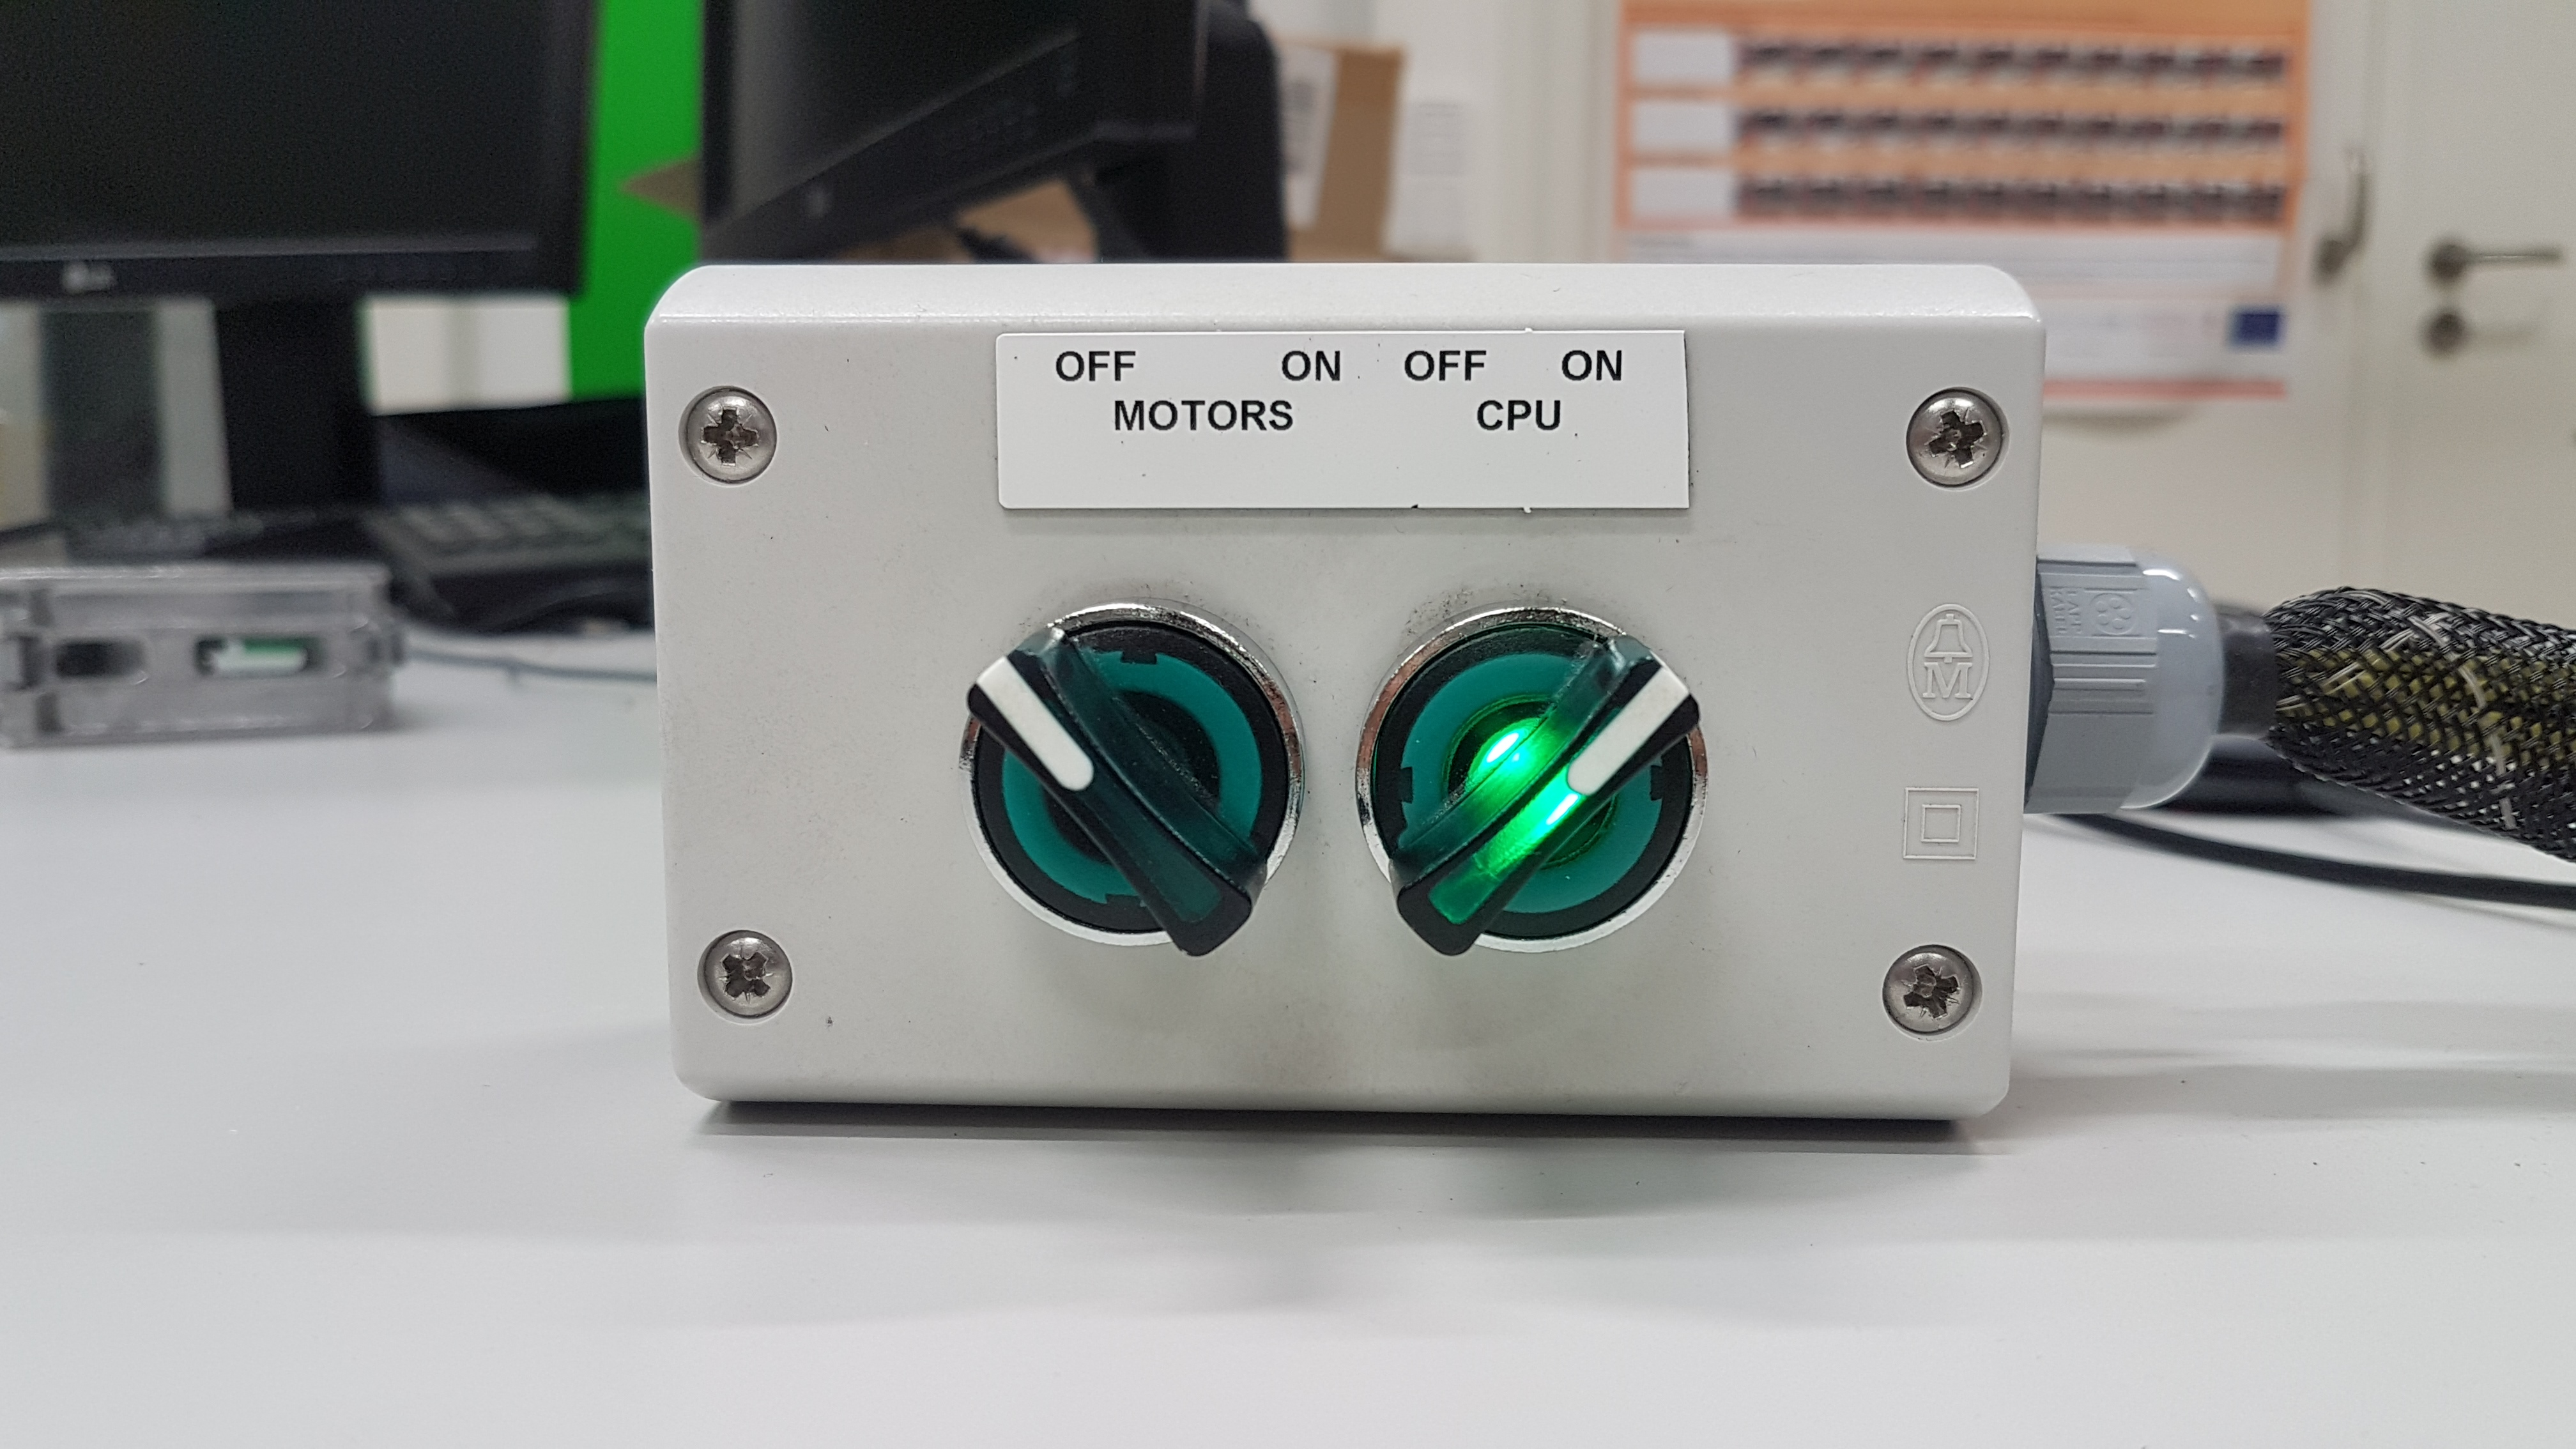
\includegraphics[scale=.04]{chapters/08_appendix/img/switch_cpu.jpg}}
		\subcaptionbox{Turn on the motors of Heicub.}%
		[.4\linewidth]{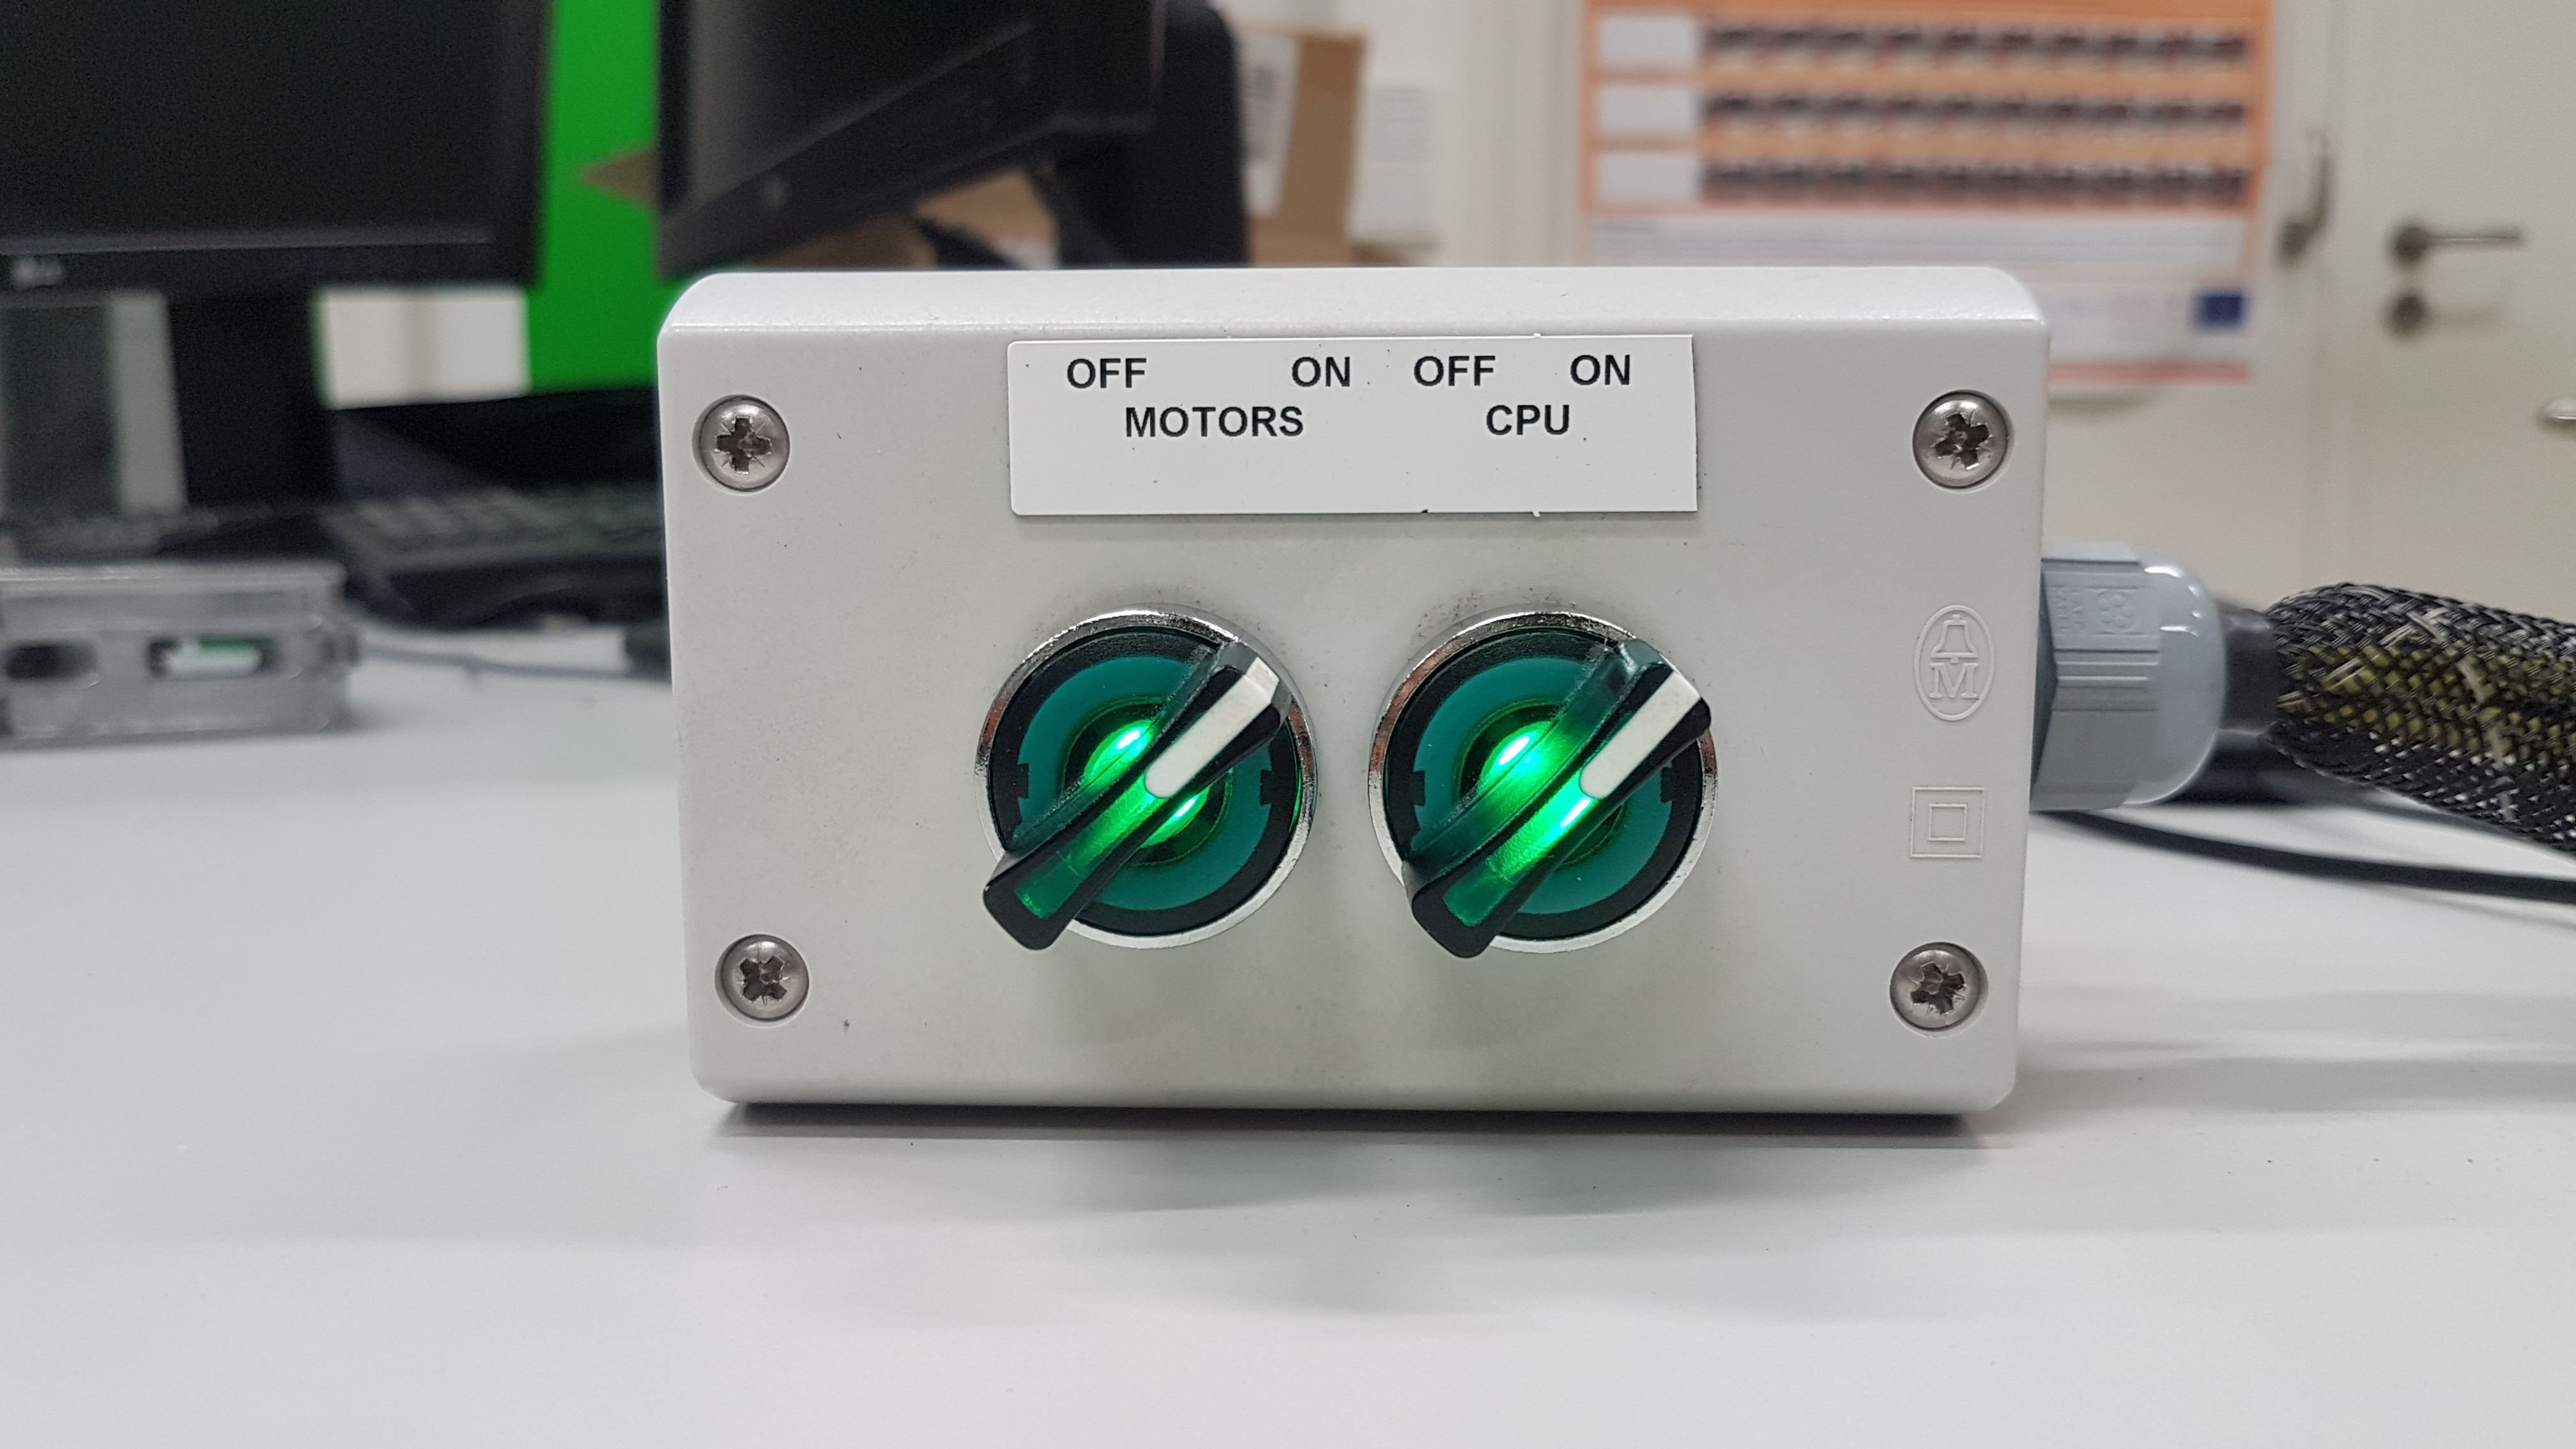
\includegraphics[scale=.04]{chapters/08_appendix/img/switch_cpu_motor.jpg}}
		\caption{Heicub's switches.}
		\label{fig::B1_cpu_motor}
	\end{figure}
	\item On the icubsrv, connect via ssh to pc104. Therefore, click on the highlighted symbol within figure \ref{fig::B1_pc104} (a). If it fails to connect, turn off the CPU, and go back to the previous step.
	\begin{figure}[h!]
		\centering
		\subcaptionbox{Run ssh to connect to pc104.}%
		[.4\linewidth]{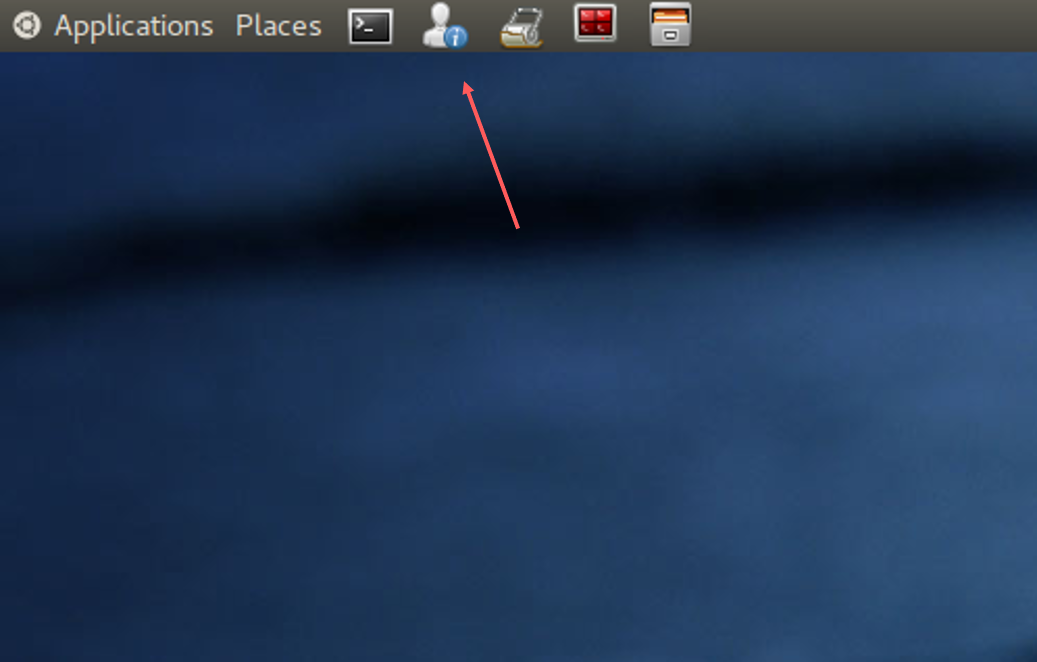
\includegraphics[scale=.326]{chapters/08_appendix/img/task_bar.png}}
		\subcaptionbox{Terminal to pc104.}%
		[.4\linewidth]{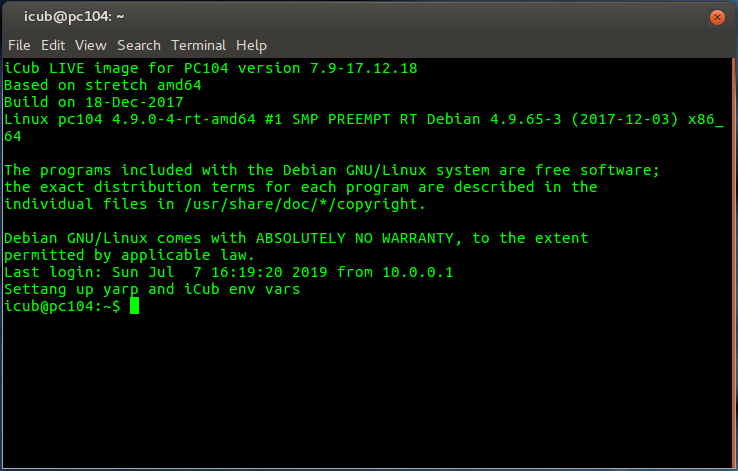
\includegraphics[scale=.22]{chapters/08_appendix/img/terminal_pc104.png}}
		\caption{Connect to pc104.}
		\label{fig::B1_pc104}
	\end{figure}
	\item Run the cluster manager from a new terminal on the icubsrv, therefore do \newline \inlinecode{}{cd /usr/local/src/robot/icub-main/build-pc104/bin}
	\newline \inlinecode{}{python icub-cluster.py}
	\item Within the cluster manager, run the YARP name server, and then YARP on all other devices (figure \ref{fig::B1_cluster} (a), then (b)).
	\begin{figure}[h!]
		\centering
		\subcaptionbox{Run the YARP nameserver.}%
		[.4\linewidth]{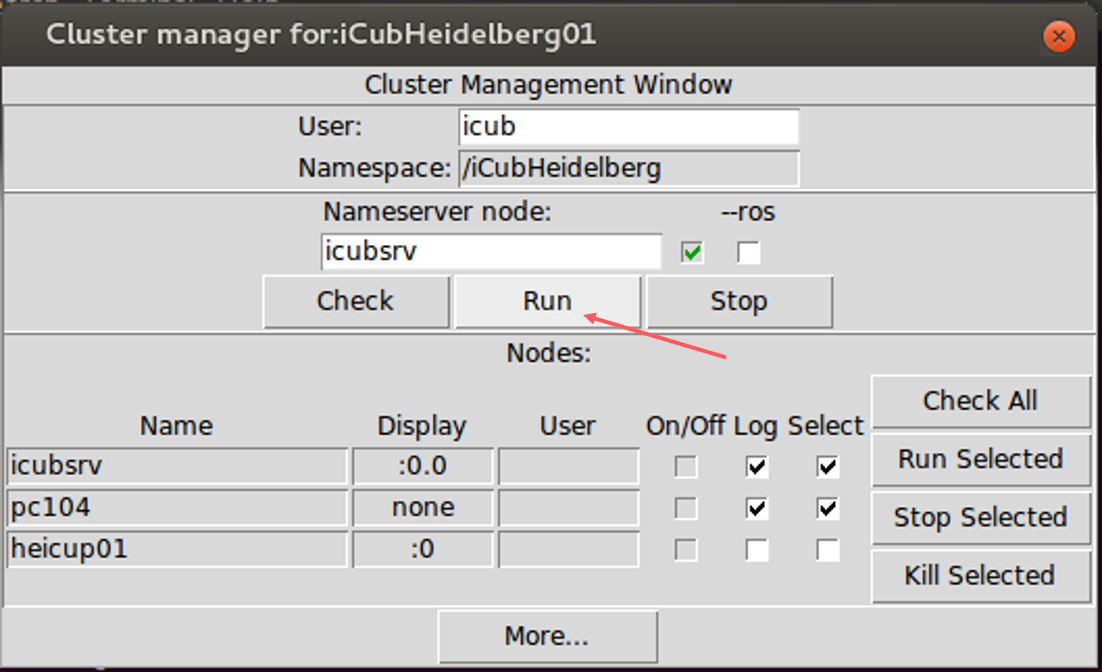
\includegraphics[scale=.3]{chapters/08_appendix/img/ran_yarp.png}}
		\subcaptionbox{Run YARP on other devices.}%
		[.4\linewidth]{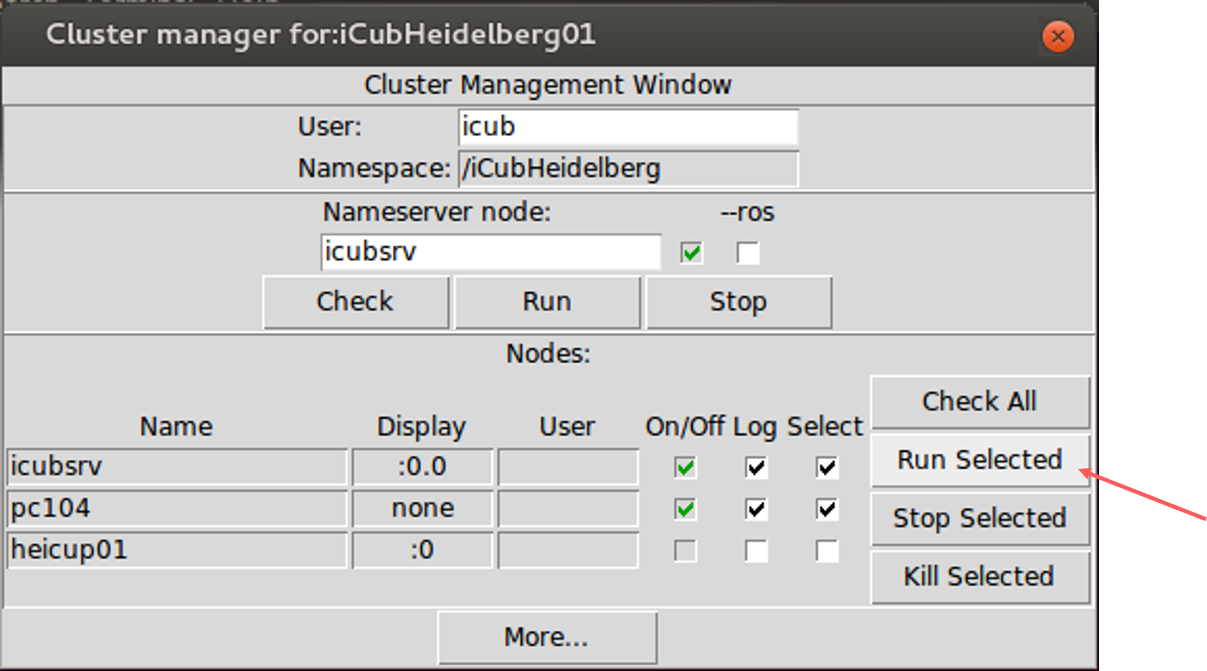
\includegraphics[scale=.3]{chapters/08_appendix/img/ran_yarp_others.png}}
		\caption{Run YARP.}
		\label{fig::B1_cluster}
	\end{figure}
	\item We can now turn on the motors and the cameras, as well as to connect our own laptop, which is explained in the following sections.
\end{enumerate}
\FloatBarrier
\subsection{Start the Motors}
\label{sec::B11_sm}
If the real robot is up and running (section \ref{sec::B1_rr}), you can now start Heicub's motors. Therefore proceed as described below.
\begin{enumerate}
	\item Turn on the motors (figure \ref{fig::B1_cpu_motor} (b)). The power suppliers should now show 13V and 40V. Wait until the blue lights at Heicub stopped blinking (figure \ref{fig::B1_blue}).
	\begin{figure}[h!]
		\centering
		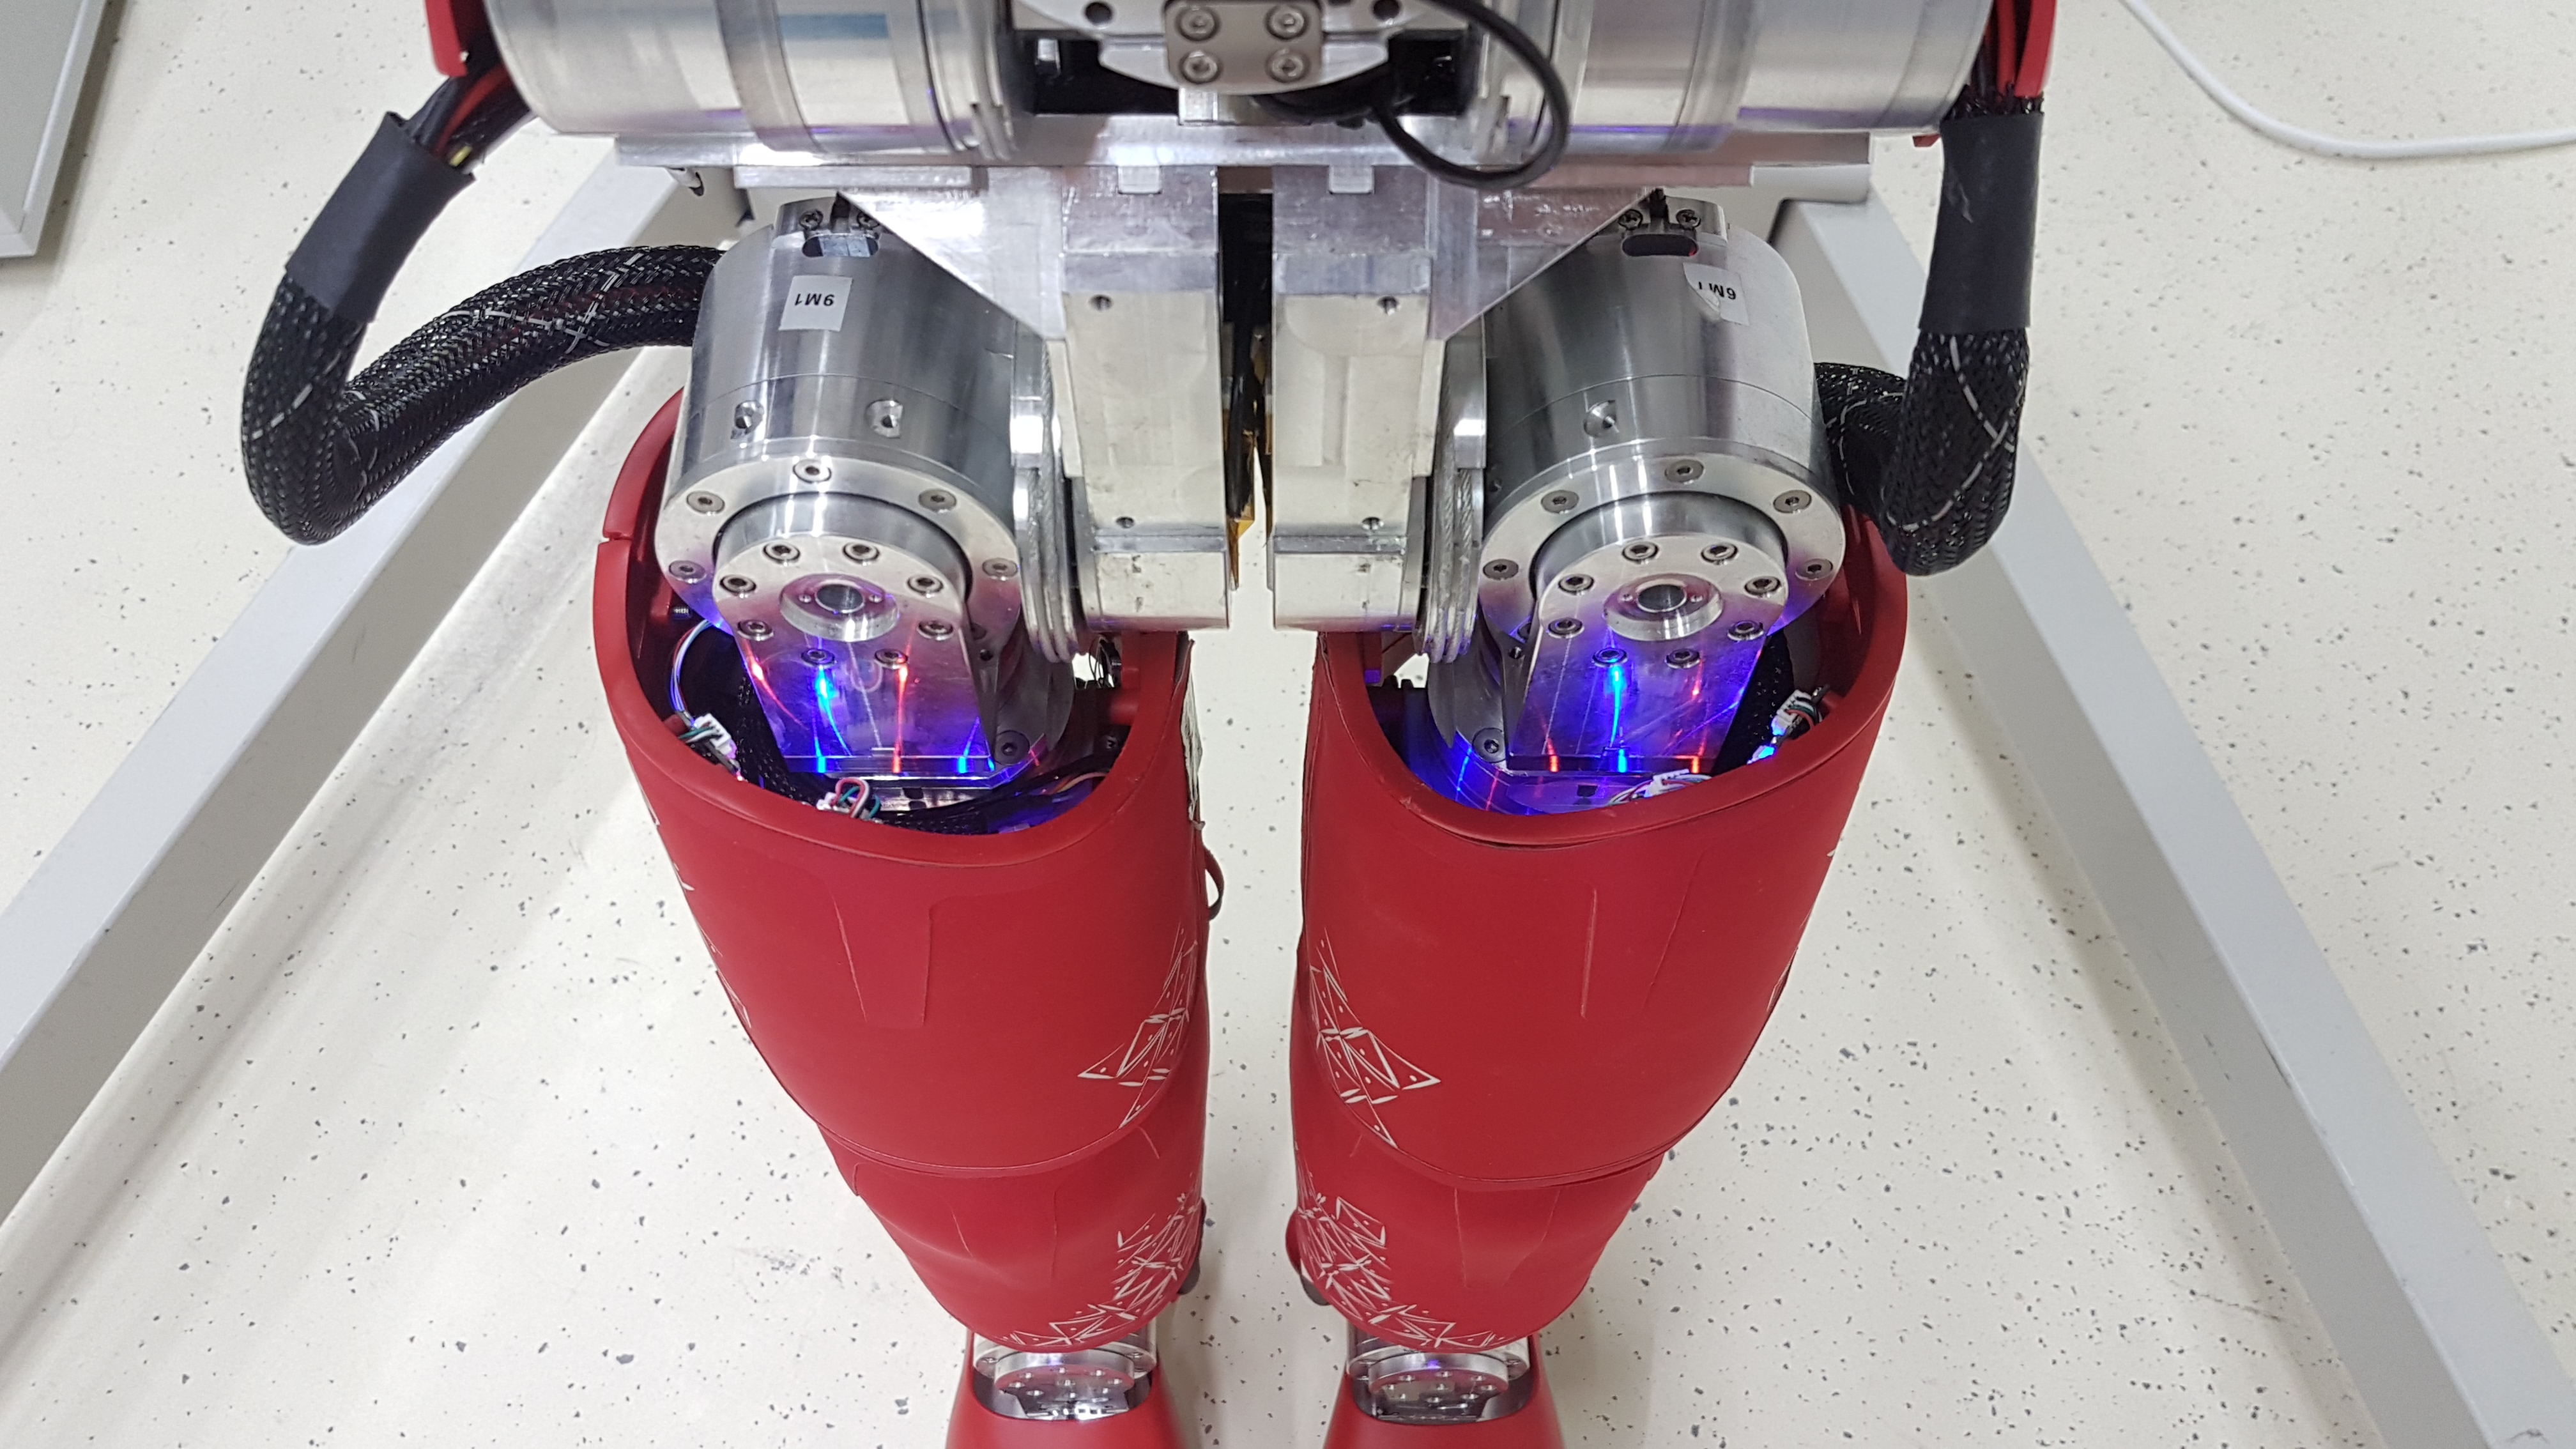
\includegraphics[scale=.04]{chapters/08_appendix/img/icub_motor_lights.jpg}
		\caption{Blue motor lights.}
		\label{fig::B1_blue}
	\end{figure}	
	\item Release the safety button (figure \ref{fig::B1_red} (b)).
	\begin{figure}[h!]
		\centering
		\subcaptionbox{Pressed safety button.}%
		[.4\linewidth]{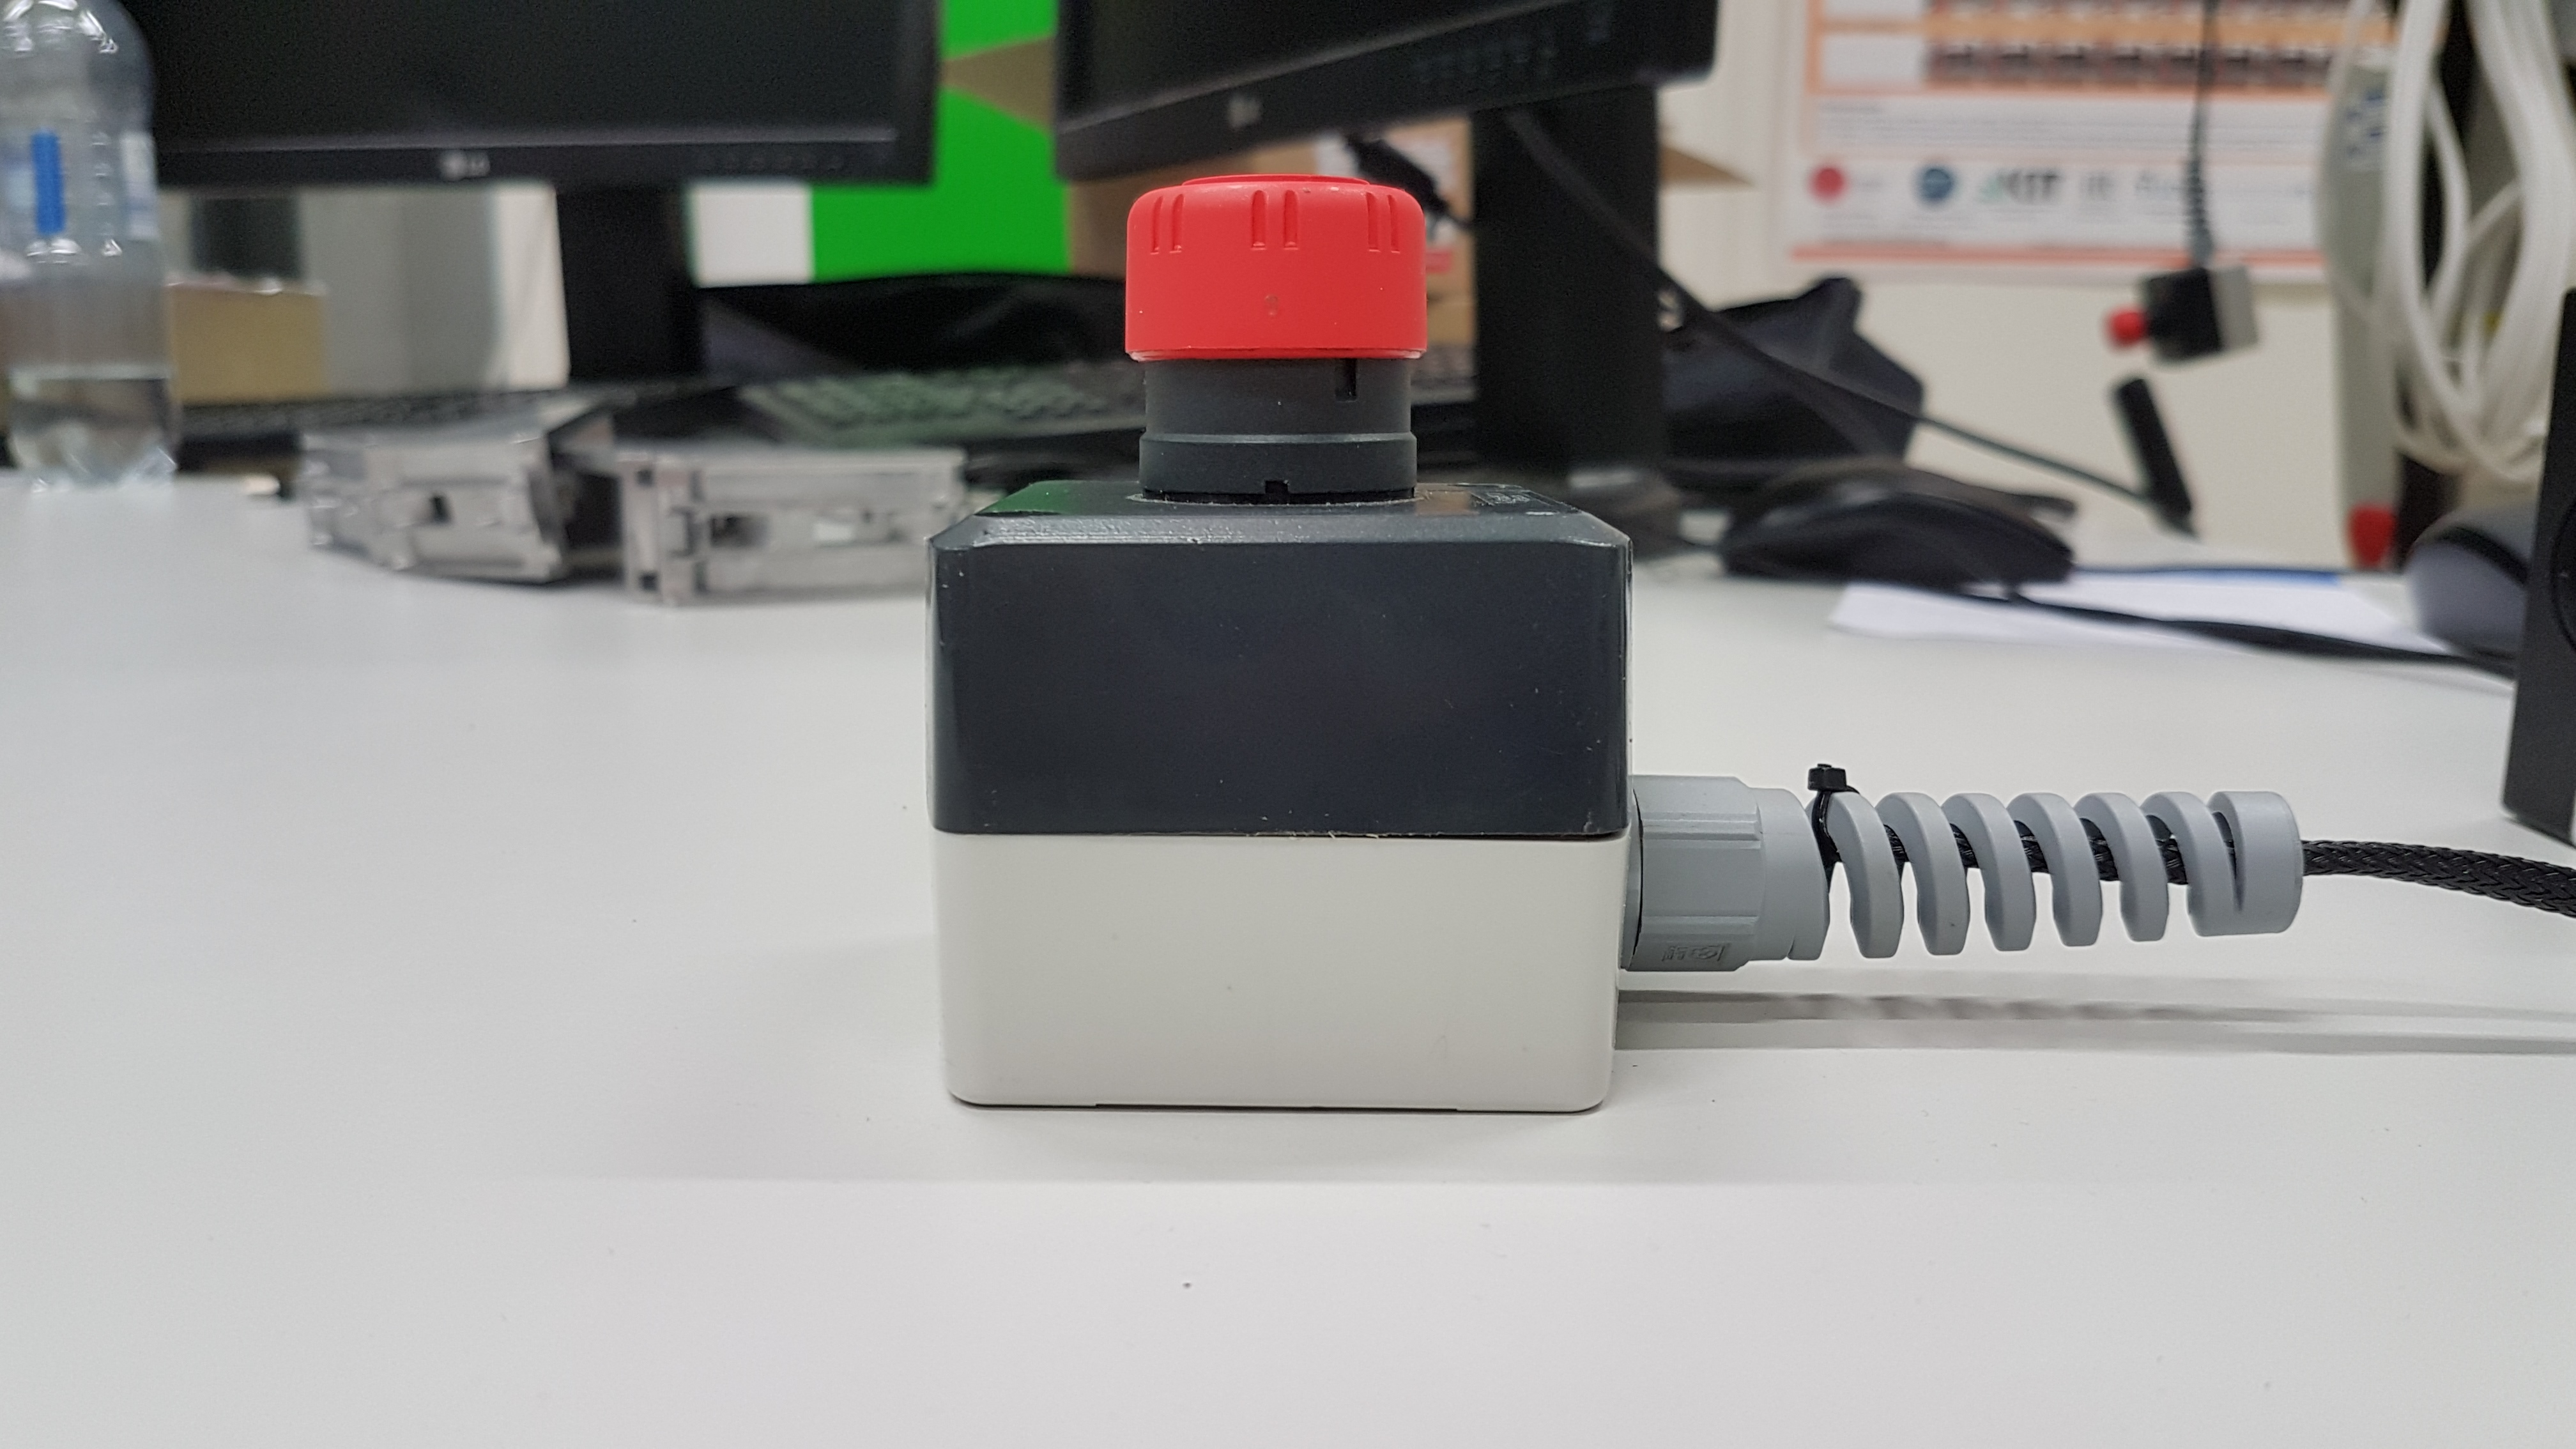
\includegraphics[scale=.04]{chapters/08_appendix/img/safety_pushed.jpg}}
		\subcaptionbox{Released safety button.}%
		[.4\linewidth]{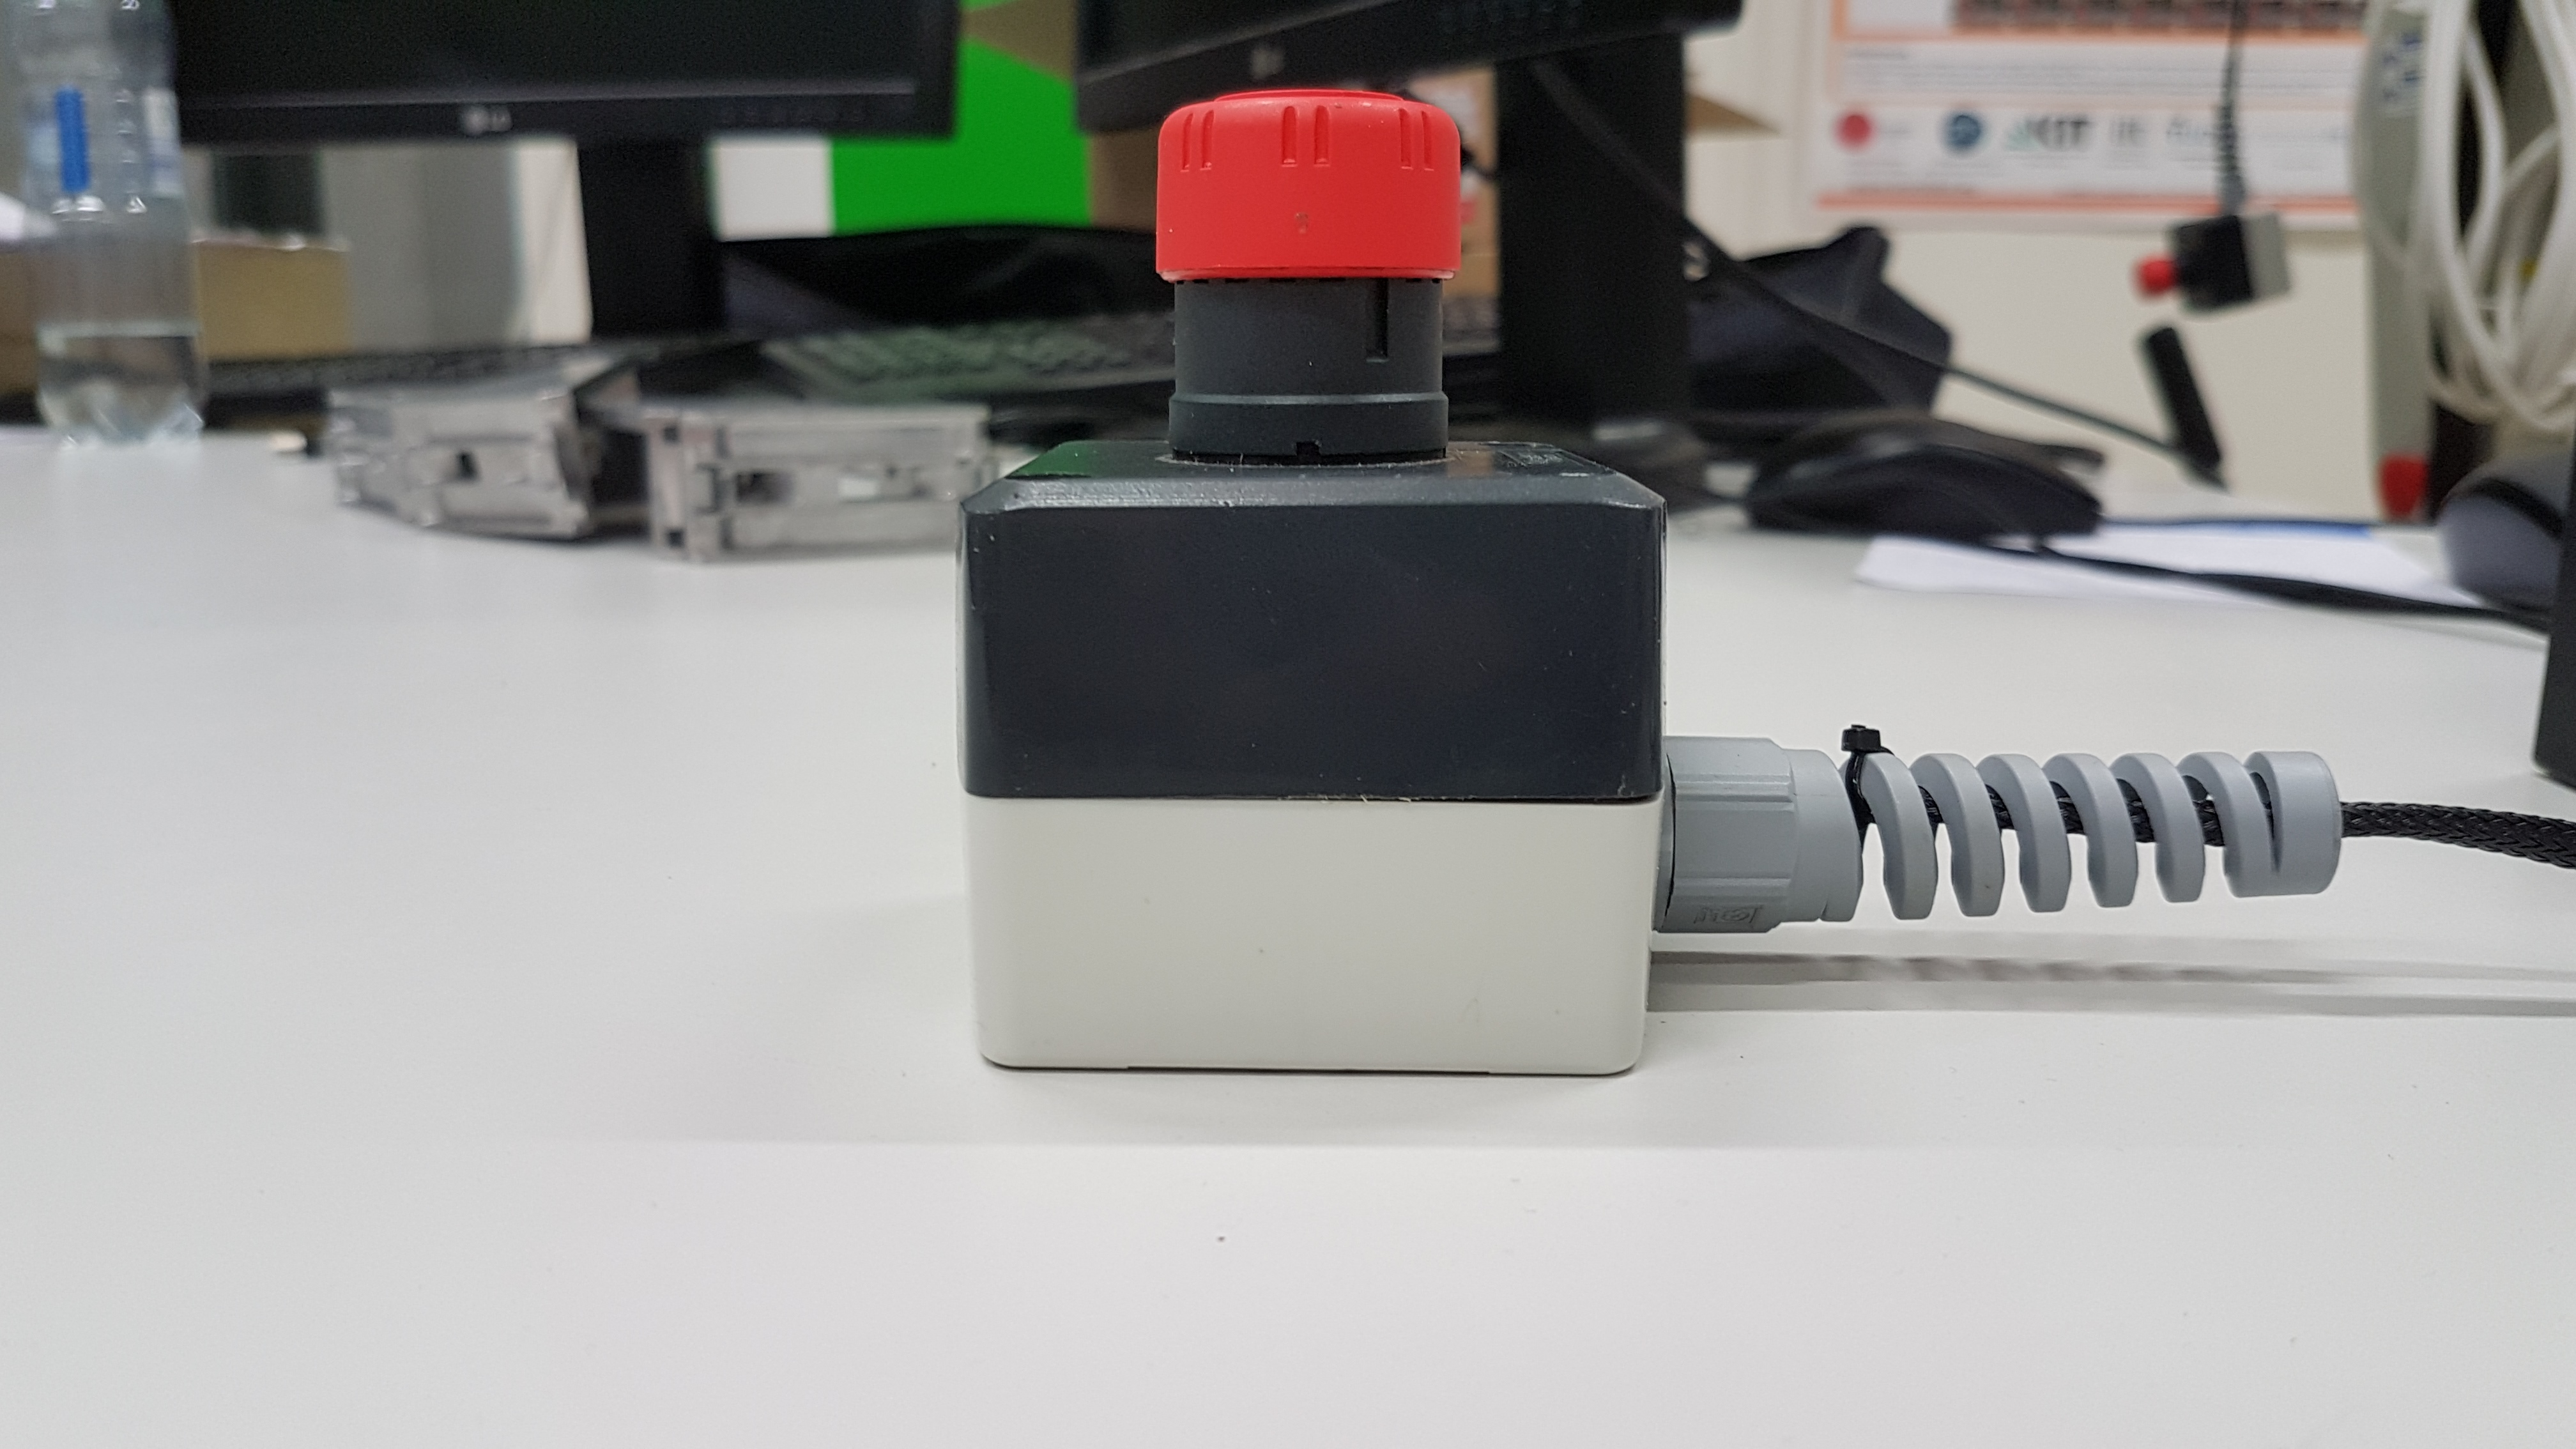
\includegraphics[scale=.04]{chapters/08_appendix/img/safety.jpg}}
		\caption{Safety button.}
		\label{fig::B1_red}
	\end{figure}
	\item Within your terminal to pc104 (figure \ref{fig::B1_pc104} (b)) run the command \newline \inlinecode{}{yarprobotinterface} \newline This will run all the motor drivers and connect them to the YARP network.
	\item If no errors occured, we can now run the yarpmotorgui to play around with the motors. This step is not necessary. To run the yarpmotorgui, open a new terminal on the icubsrv, and run the command \newline \inlinecode{}{yarpmotorgui} (figure \ref{fig::B11_gui} (a)) \newline Then, press \inlinecode{}{OK}. The motors can now be manipulated from within the GUI (figure \ref{fig::B11_gui} (b)), e.g. by clicking on the house, which will bring all motors to the home position.
	\begin{figure}[h!]
		\centering
		\subcaptionbox{Run the yarpmotorgui.}%
		[.4\linewidth]{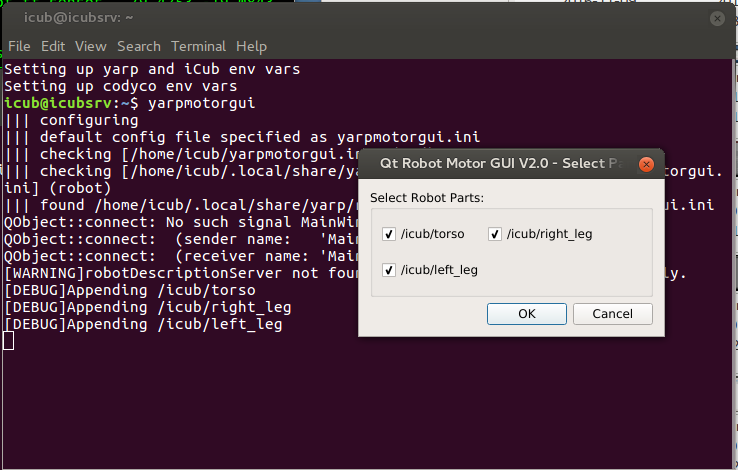
\includegraphics[scale=.22]{chapters/08_appendix/img/yarpmotorgui_ok.png}}
		\subcaptionbox{The yarpmotorgui.}%
		[.4\linewidth]{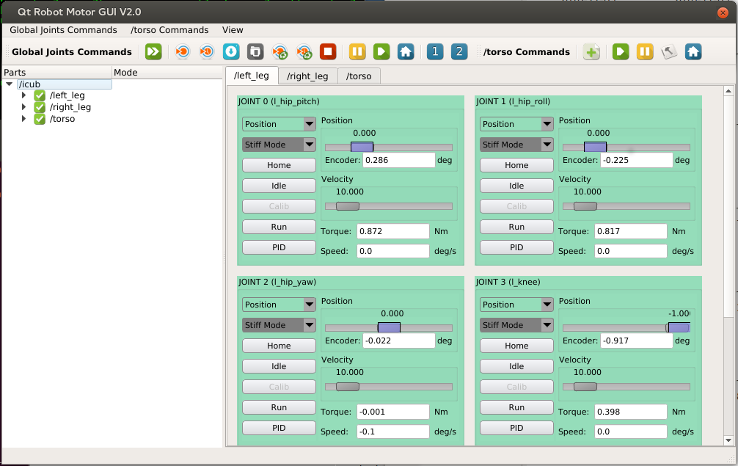
\includegraphics[scale=.22]{chapters/08_appendix/img/yarpmotorgui_api.png}}
		\caption{Accessing the motors.}
		\label{fig::B11_gui}
	\end{figure}
	\item The motors may need to be calibrated when the robot runs for a long time. Therefore, lift up the robot, and bring it to the home position via the yarpmotorgui. Then, start a new terminal on pc104 and run the command \newline \inlinecode{}{yarp rpc /wholeBodyDynamics/rpc} \newline In the interface that will open up, type \newline \inlinecode{}{calib all 300}. 
\end{enumerate}
\FloatBarrier
\subsection{Start the Cameras}
\label{sec::B12_sc}
If the real robot is up and running (section \ref{sec::B1_rr}), you can now start Heicub's cameras. Therefore, proceed as described below.
\begin{enumerate}
	\item Within a new terminal to pc104 (figure \ref{fig::B1_pc104} (a)), do \newline \inlinecode{}{cd ./local/share/yarp/robots/iCubHeidelberg01/camera}\newline Then, start the camera via \newline \inlinecode{}{yarpdev --from dragonfly2_config_left.ini}\newline This will run the left camera and connect it to the YARP network. Repeat the above steps for the right camera, but replace left by right within the \inlinecode{}{.ini} file.
	\item If no errors occured, we can now run a yarpview to see what Heicub sees. This step is not necessary. To run a yarpview, open a new terminal on the icubsrv, and run the command \newline \inlinecode{}{yarpview} (figure \ref{fig::B12_yarpview} (a)) \newline Then, connect a camera to the yarpview. Therefore, open a new terminal on the icubsrv and run the command \newline \inlinecode{}{yarp connect /icub/cam/left /yarpview/img:i} (figure \ref{fig::B12_yarpview} (b)) \newline You should now see an image.
	\begin{figure}[h!]
		\centering
		\subcaptionbox{Run a yarpview.}%
		[.4\linewidth]{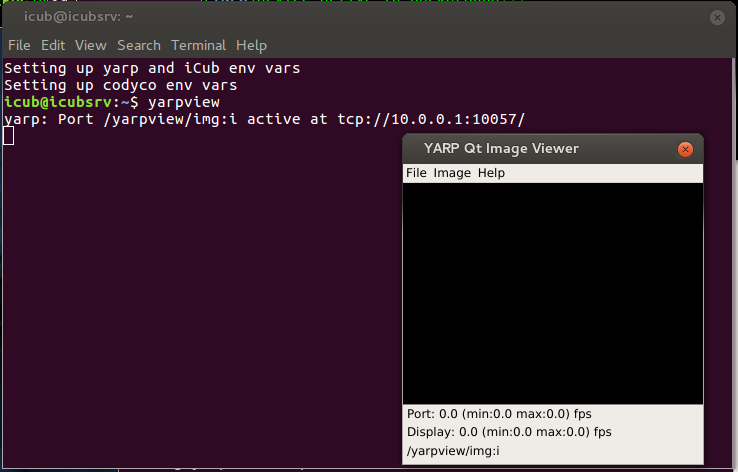
\includegraphics[scale=.22]{chapters/08_appendix/img/yarpview.png}}
		\subcaptionbox{Connect a camera to the yarpview.}%
		[.4\linewidth]{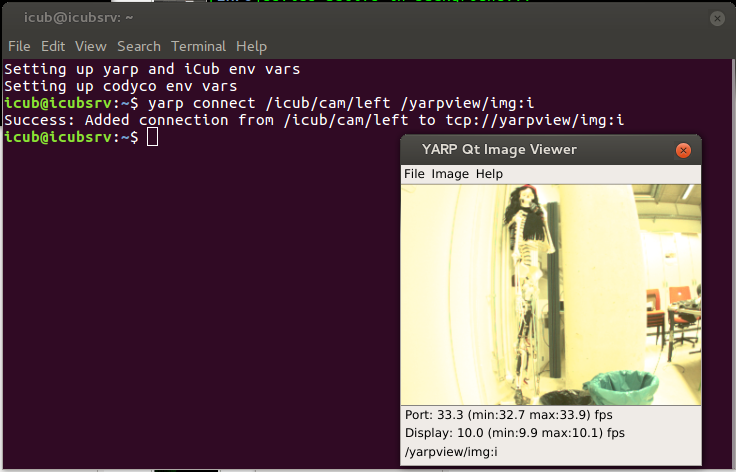
\includegraphics[scale=.22]{chapters/08_appendix/img/connect_yarpview.png}}
		\caption{Accessing the cameras.}
		\label{fig::B12_yarpview}
	\end{figure}
\end{enumerate}
\FloatBarrier
\subsection{Connect your own Laptop}
Make sure you installed YARP, as described in section \ref{sec::A5_tp}. You can then connect your own laptop via ethernet to the same network as Heicub. Therefore, proceed as described below.
\begin{enumerate}
	\item  Connect a LAN cable to the switch to which the icubsrv is connected as well (figure \ref{fig::B1_icubsrv}). You will then get assigned an IP address within the same domain as the icubserver, such as \inlinecode{}{10.0.0.x}. Check this by running \inlinecode{}{ifconfig}. The IP address of the icubsrv is \inlinecode{}{10.0.0.1}, while that of the pc104 is \inlinecode{}{10.0.0.2}.
	\item  Check the connection by pinging the icubsrv via \inlinecode{}{ping 10.0.0.1}. If this works, skip this point, otherwise you can create a manual connection.  Therefore, search for \inlinecode{}{Network Connections} among your applications and open it. Then, click \inlinecode{}{Add}. If it is not set already, check the hardware address by running \inlinecode{}{ifconfig}, it should show something similar to \inlinecode{}{HWaddr 9C:EB:E8:B2:AB:27}, choose this as your device. Then go to IPv4 settings and set the IP address to \inlinecode{}{10.0.0.3}, the netmask to \inlinecode{}{24}, and the gateway to \inlinecode{}{10.0.0.255}. Then press save.
	\item If you connected successfully, open a terminal on your device and run \newline \inlinecode{}{yarp detect --write} \newline If it does not find the running yarpserver, manually configure the connection via the following commands from a terminal \newline \inlinecode{}{yarp conf 10.0.0.1 1000} \newline \inlinecode{}{yarp namespace /iCubHeidelberg} \newline \inlinecode{}{yarp detect}
\end{enumerate}
\FloatBarrier
\section{Simulated Robot Start-up}
\label{sec::B2_ss}
Make sure you installed Gazebo, YARP, and the Gazebo YARP plugins as described in section \ref{sec::A5_tp}. Also, you need to have the simulation model installed, which is described in section \ref{sec::A4_sm}. When these requirements are satisfied, then proceed as described below.
\begin{enumerate}
	\item Open a terminal and start YARP via \newline \inlinecode{}{yarpserver --write} \newline
	\item Open another terminal and start Gazebo via \newline \inlinecode{}{gazebo -s libgazebo_yarp_clock.so}\newline The clock library will thereby synchronize the YARP clock, and the Gazebo clock.
	\item  In Gazebo, go to the \inlinecode{}{Insert} bar, and insert \inlinecode{}{heicub_without_weights}.
\end{enumerate}
\FloatBarrier
\section{Start the Pattern Generator}
\label{sec::B3_sp}
Make sure you installed the pattern generator library as described in section \ref{sec::A1_pg}. The robot needs to be running, either in real (section \ref{sec::B1_rr}, and section \ref{sec::B11_sm}) or in simulation (section \ref{sec::B2_ss}). By construction, the start-up procedure for the simulation and the real robot is the same. You can choose to control the robot via the terminal, or the provided Android app. Both possibilities are described below in section \ref{sec::B31_terminal}, and section \ref{sec::B32_app}, respectively.
\FloatBarrier
\subsection{Control via the Terminal}
\label{sec::B31_terminal}
The terminal user interface comes with the pattern generator, so there is no additional software that needs to be installed. Proceed as described below.
	\begin{enumerate}
		\item Open a new terminal and go to the shell scripts within the pattern generator folder via \newline \inlinecode{}{cd nmpc\_pattern\_generator/sh} \newline On the icubsrv, this folder is located at \inlinecode{}{/usr/local/src/robot}. Then, run the keyboard user interface via \newline \inlinecode{}{sh run\_keyboard\_user\_interface.sh}
	\item The shell script will then ask you whether to run the robot in real or in simulation, write \inlinecode{}{y} or \inlinecode{}{n} and press enter (figure \ref{fig::B31_keyboard} (a)).
	\item The shell script will then ask you for the mode to run in. Write \inlinecode{}{uc} and press enter (figure \ref{fig::B31_keyboard} (a)).
	\item The user interface should now show up and explain how to control the robot (figure \ref{fig::B31_keyboard} (b)).
	\begin{figure}[h!]
		\centering
		\subcaptionbox{Select the mode to run the pattern generator in.}%
		[.4\linewidth]{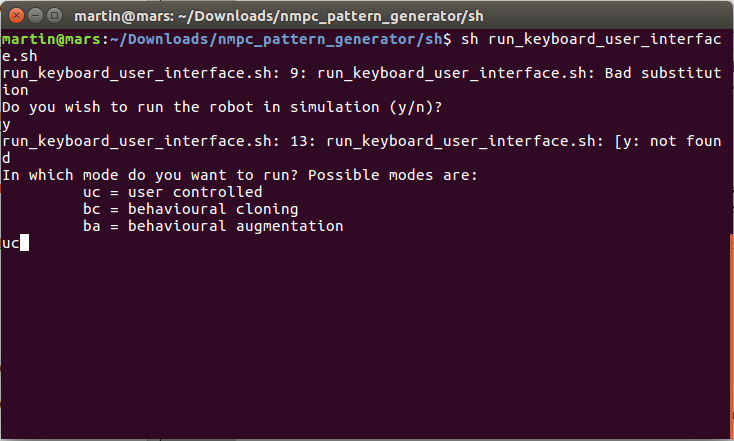
\includegraphics[scale=.22]{chapters/08_appendix/img/keyboard_mode.png}}
		\subcaptionbox{Keyboard user interface.}%
		[.4\linewidth]{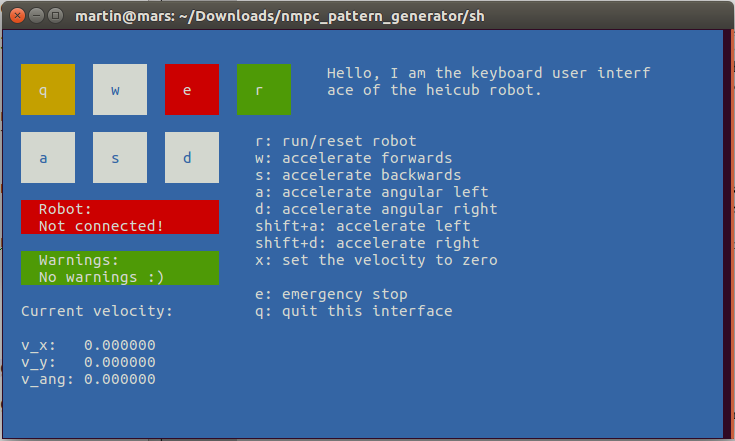
\includegraphics[scale=.22]{chapters/08_appendix/img/keyboard_interface.png}}
		\caption{Run the keyboard user interface.}
		\label{fig::B31_keyboard}
	\end{figure}
\end{enumerate}
\FloatBarrier
\subsection{Control via the Android Joystick App}
\label{sec::B32_app}
Make sure you installed the Android joystick app as described in section \ref{sec::A2_aa}. Proceed as described below.
\begin{enumerate}
	\item Open a hotspot from your phone and connect the icubsrv or your laptop to it.
	\item Open a new terminal and go to the shell scripts within the pattern generator folder via
	\newline \inlinecode{}{cd nmpc\_pattern\_generator/sh}\newline
	On the icubsrv, this folder is located at \inlinecode{}{/usr/local/src/robot}. Then, run the app user interface via
	\newline \inlinecode{}{sh run\_app\_user\_interface.sh}
	\item The shell script will then ask you whether to run the robot in real or in simulation, write \inlinecode{}{y} or \inlinecode{}{n} and press enter (figure \ref{fig::B32_app} (a)).
	\item The user interface should now show up and explain how to control the robot (figure \ref{fig::B32_app} (b)).
	\begin{figure}[h!]
		\centering
		\subcaptionbox{Select the mode to run the pattern generator in.}%
		[.4\linewidth]{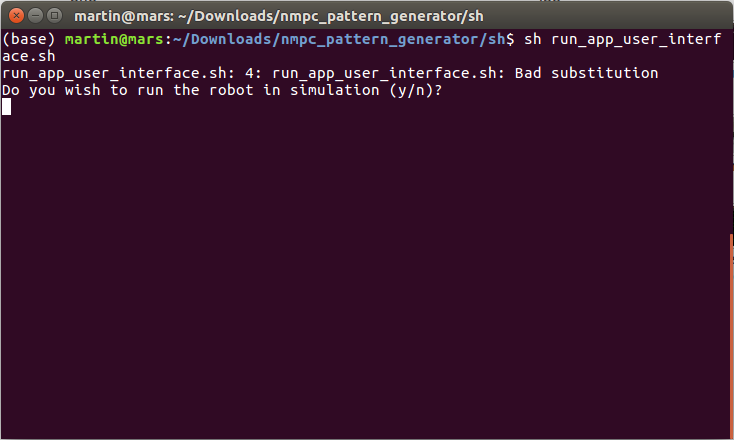
\includegraphics[scale=.22]{chapters/08_appendix/img/app_mode.png}}
		\subcaptionbox{App user interface.}%
		[.4\linewidth]{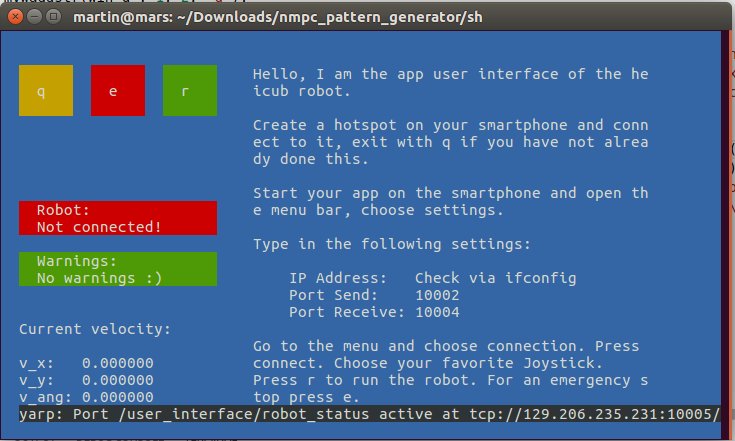
\includegraphics[scale=.22]{chapters/08_appendix/img/app_interface.png}}
		\caption{Run the app user interface.}
		\label{fig::B32_app}
	\end{figure}
	\item Open the Android app on your smartphone. Within the app, choose settings from the navigation drawer (figure \ref{fig::B32_app_settings} (a)). In the settings activity (figure \ref{fig::B32_app_settings} (b)), choose the IP address and the ports as proposed by the app user interface (figure \ref{fig::B32_app} (b)). 
	\begin{figure}[h!]
		\centering
		\subcaptionbox{Navigation drawer.}%
		[.3\linewidth]{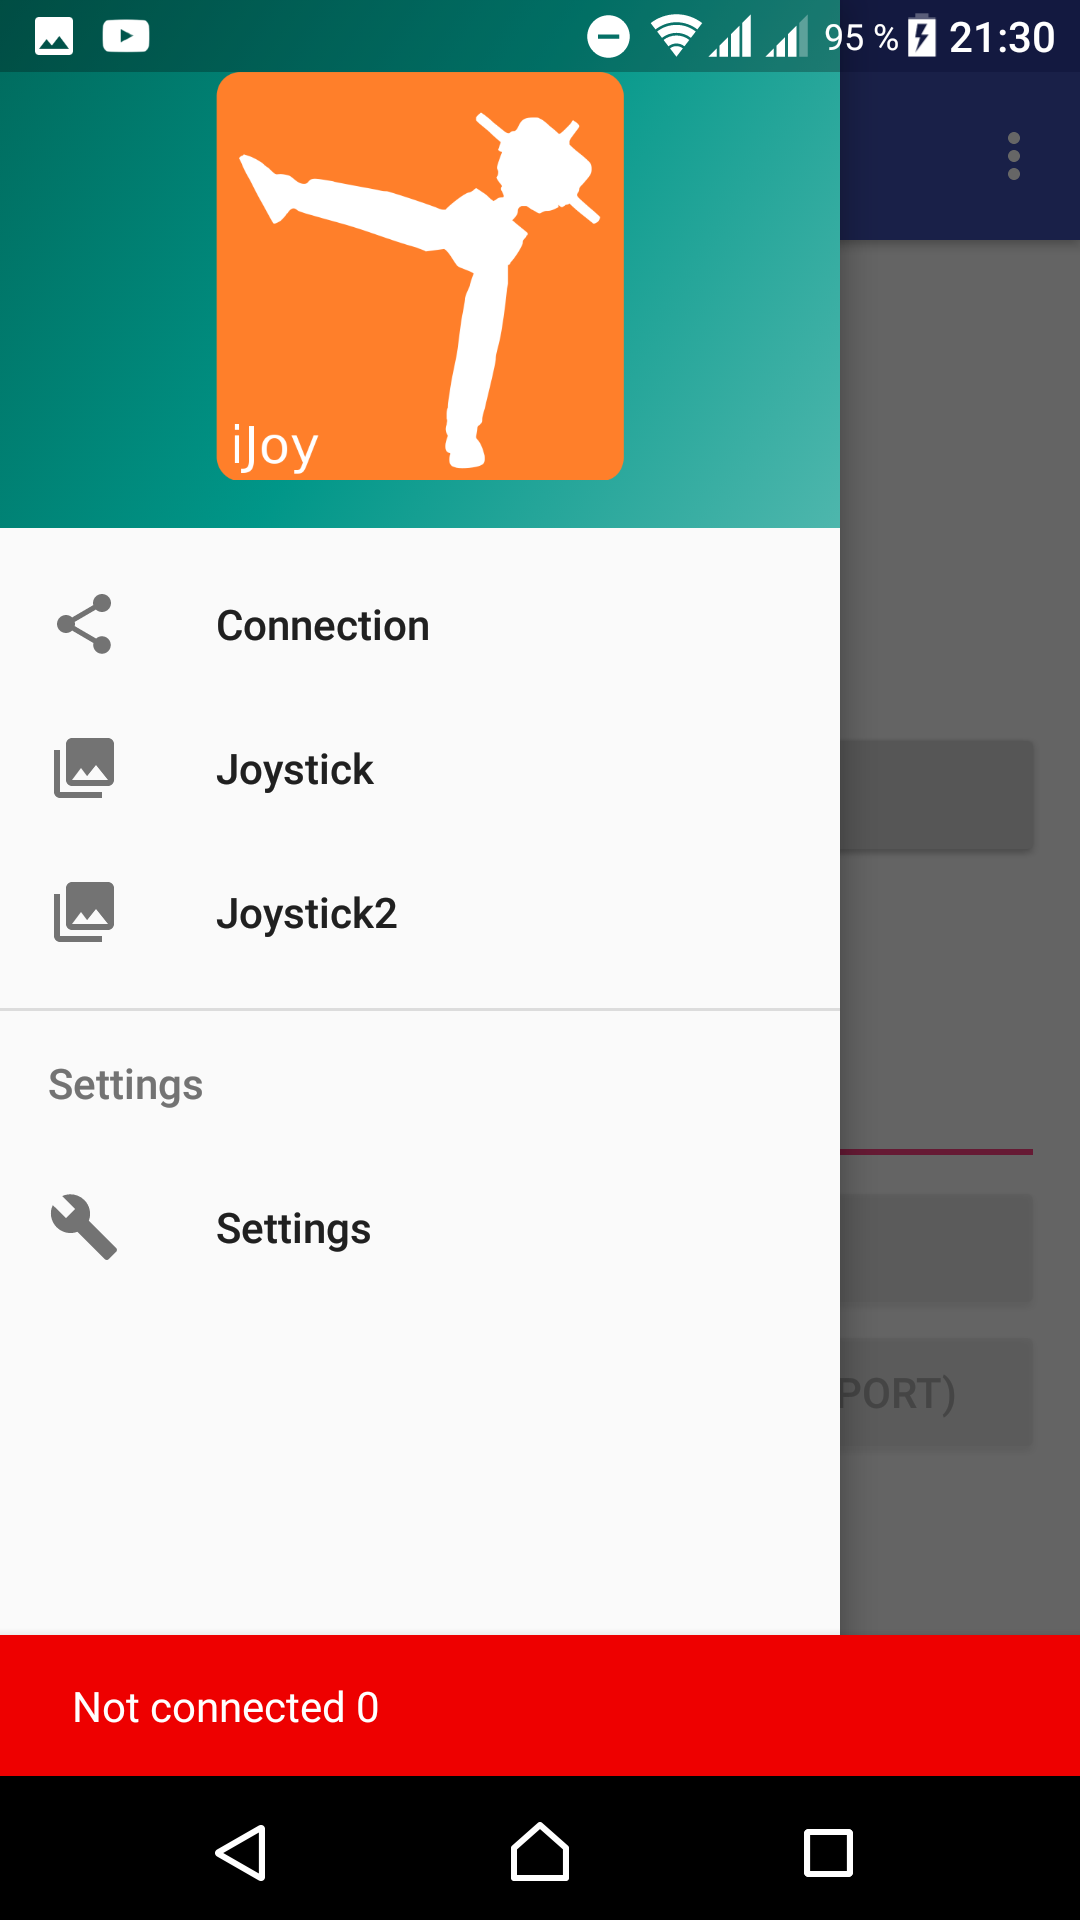
\includegraphics[scale=.08]{chapters/08_appendix/img/slider.png}}
		\subcaptionbox{Settings activity.}%
		[.3\linewidth]{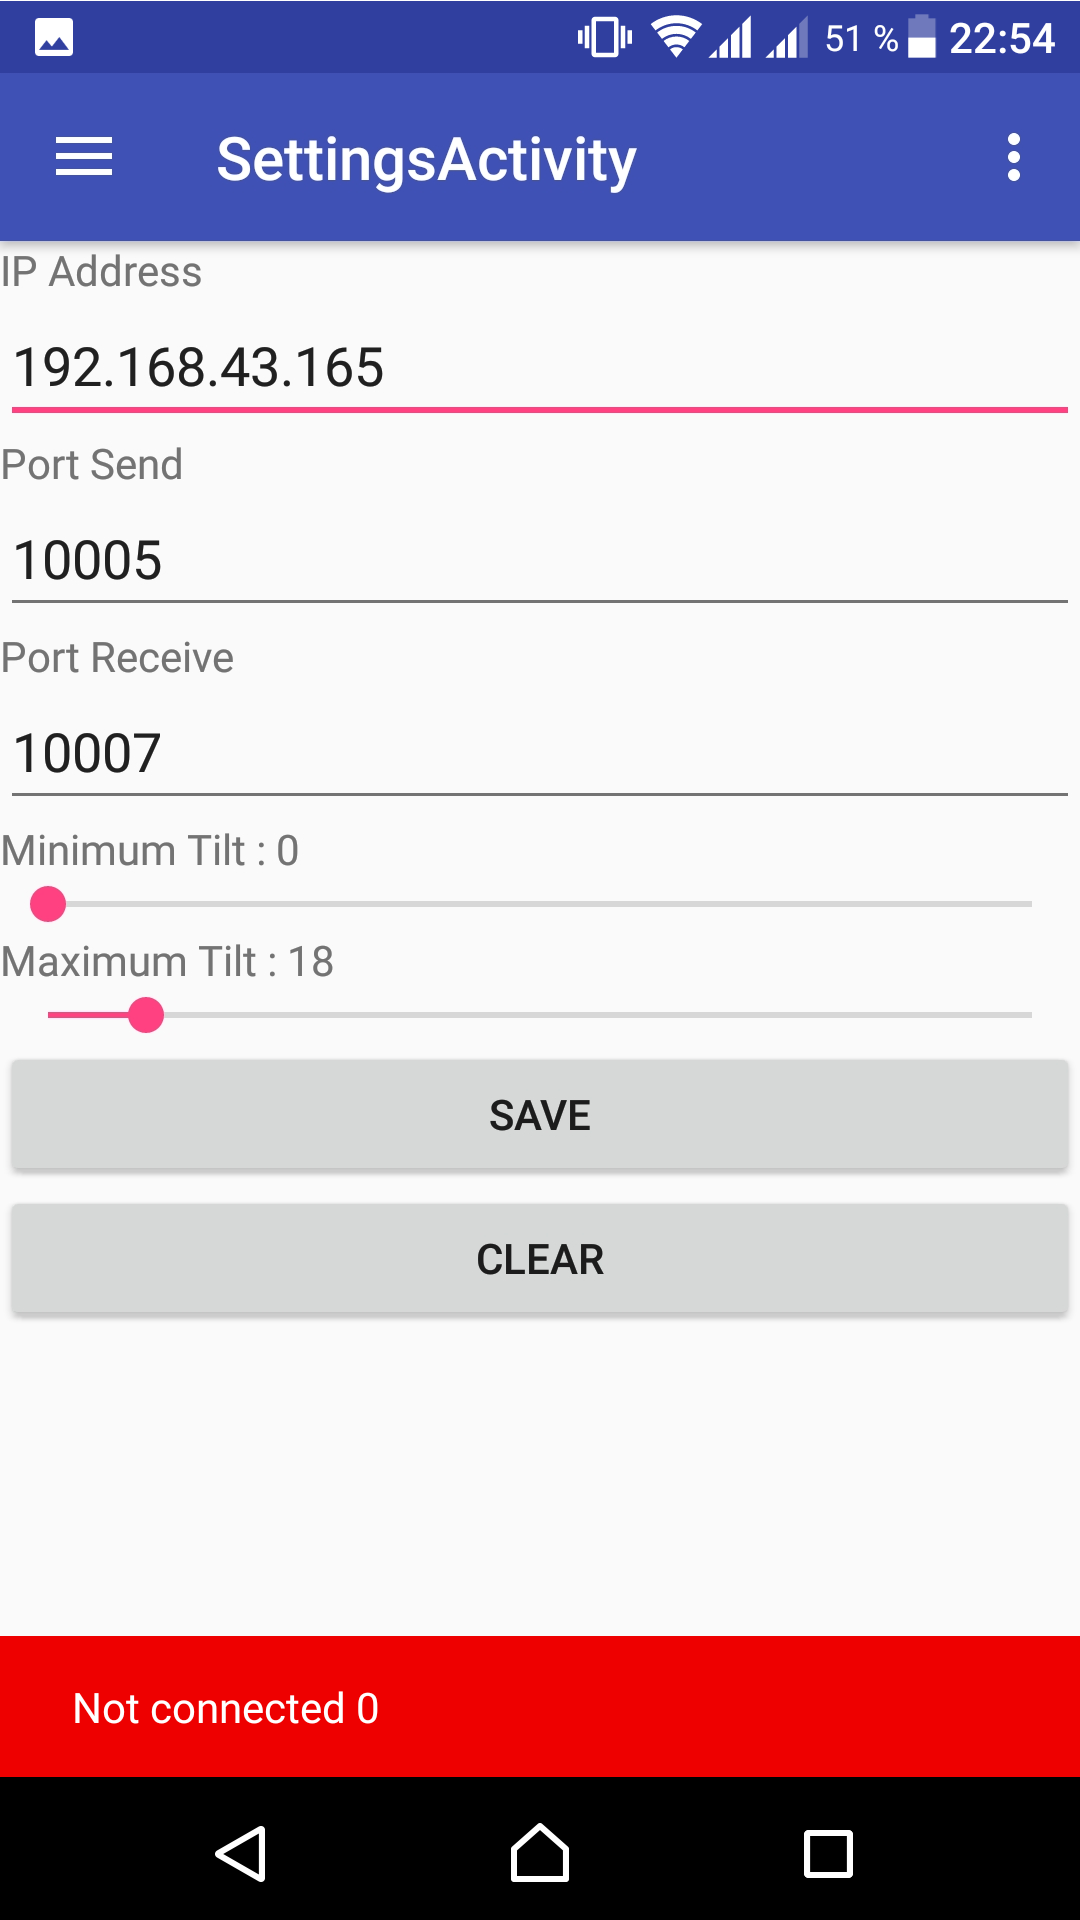
\includegraphics[scale=.08]{chapters/08_appendix/img/settings.png}}
		\subcaptionbox{Connect activity.}%
		[.3\linewidth]{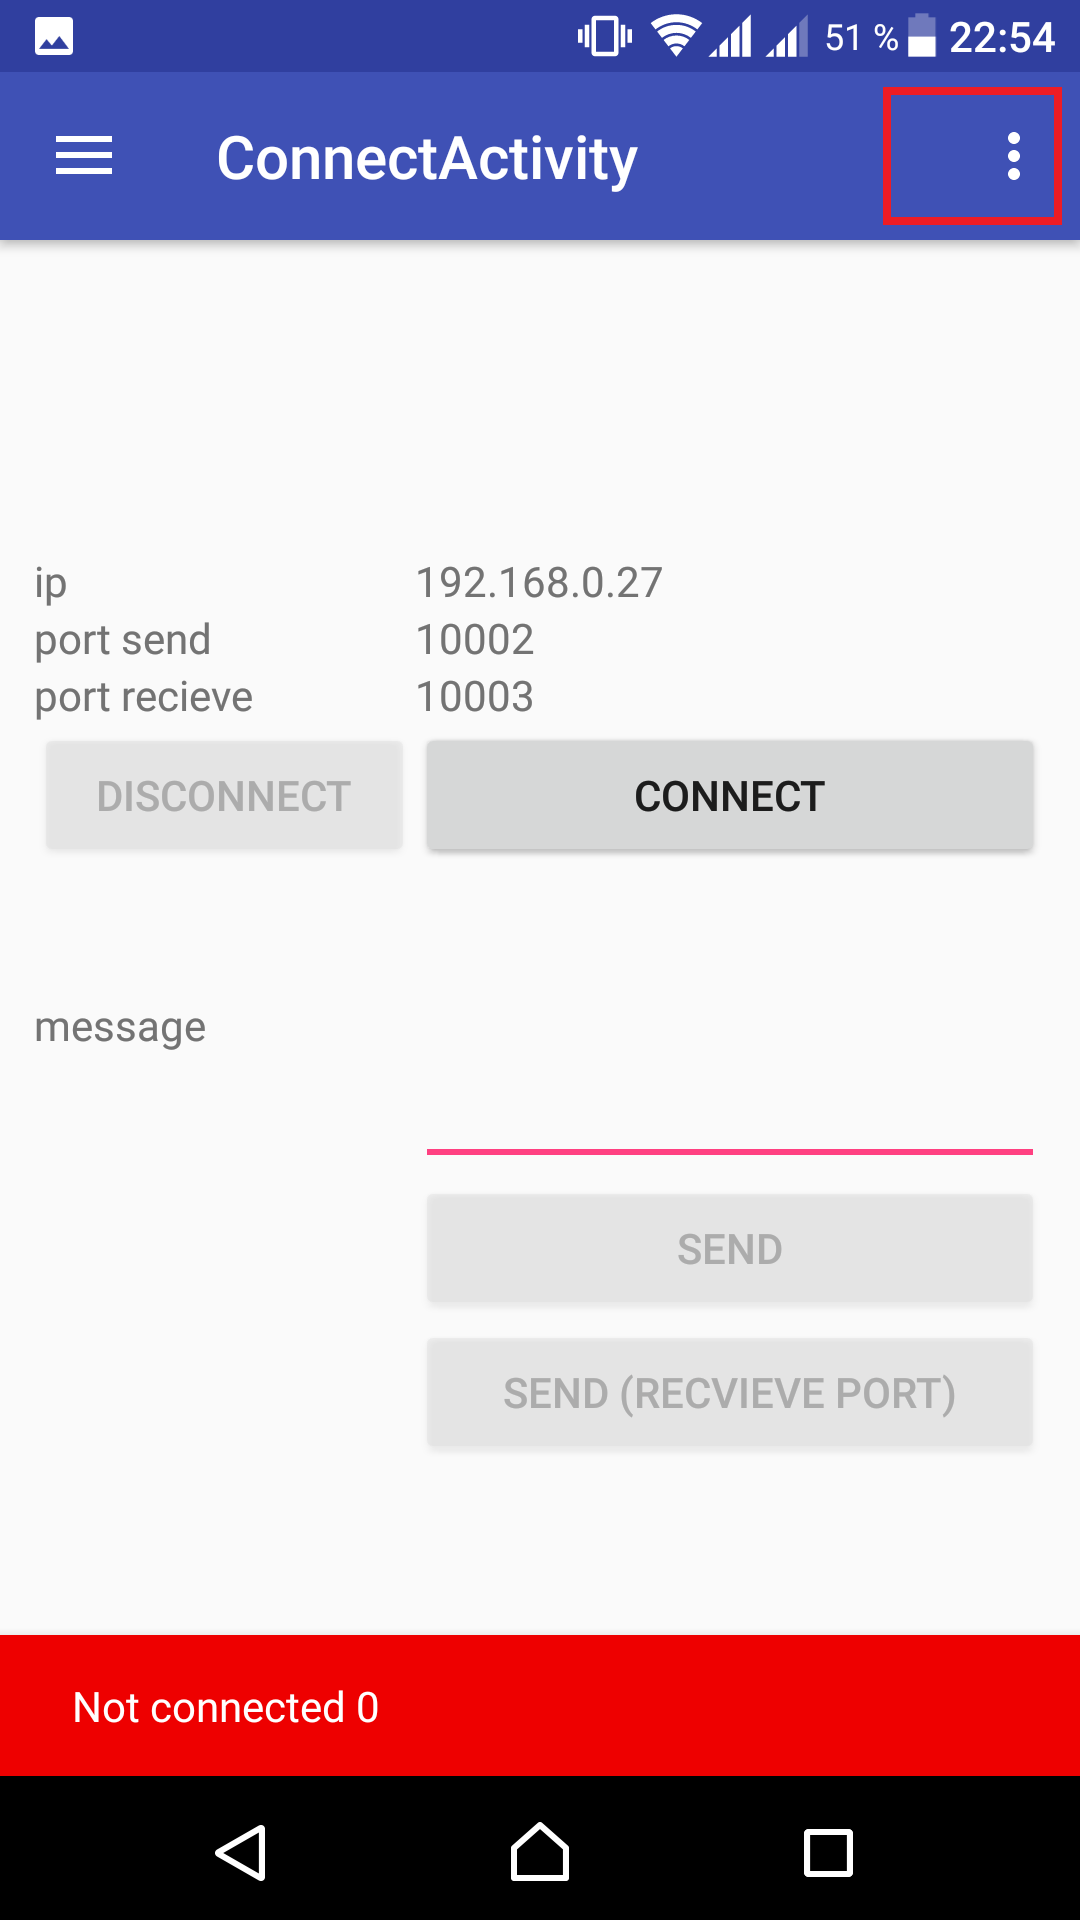
\includegraphics[scale=.107]{chapters/08_appendix/img/connect_settings.png}}
		\caption{Connect the app to the computer.}
		\label{fig::B32_app_settings}
	\end{figure}
	\item Now go to the connection activity (figure \ref{fig::B32_app_settings} (c)), and press connect. You should now be connected.
	\item Go to the app user interface on the laptop (figure \ref{fig::B32_app} (b)), and press \inlinecode{}{r} to run the pattern generator.
	\item Within the navigation drawer, choose from one of two joysticks to control the robot.
\end{enumerate}
\FloatBarrier
\section{Start the Behavioral Augmentation Demo}
\label{sec::B4_ba}
There is a trained neural network available on heicub01 to run a demonstration of the behavioral augmentation as trained in section \ref{sec::42_ab}. The network will navigate Heicub towards a fire extinguisher and look around if it does not see one. Make sure the robot and its cameras are running (section \ref{sec::B1_rr}, section \ref{sec::B11_sm}, and section \ref{sec::B12_sc}). Proceed as described below.
\begin{enumerate}
	\item Login to heicub01, username is \inlinecode{}{icub}, ask someone at the ORB for the password.%password it \inlinecode{}{icubheidelberg01}.
	\item Make sure that YARP is running on heicub01 (figure \ref{fig::B1_cluster} (b)). Therefore, select heicub01 and click \inlinecode{}{Run Selected}.
	\item On heicub01, open a new terminal and go to the shell scripts within the pattern generator folder via \newline \inlinecode{}{cd /home/icub/Documents/nmpc\_pattern\_generator/sh}
	\newline Then run the keyboard user interface with
	\newline \inlinecode{}{sh run\_keyboard\_user\_interface.sh}
	\item The shell script will then ask you whether to run the robot in real or in simulation, write \inlinecode{}{n} and press enter (figure \ref{fig::B31_keyboard} (a)).
	\item The shell script will then ask you for the mode to run in. Write \inlinecode{}{ba} and press enter.
	\item The user interface should now show up (figure \ref{fig::B31_keyboard} (b)). Press \inlinecode{}{r} to run the pattern generator. The robot will now be controlled by the trained neural network.
\end{enumerate}
\FloatBarrier
\section{Real Robot Shutdown}
Before you shut down the robot, make sure it is in a safe position, that is, lift it up. Proceed as described below.
\begin{enumerate}
	\item Lift the robot from the floor.
	\item Close all running applications. \inlinecode{}{Ctrl+C} the yarprobotinterface and the camera interfaces.
	\item Type \inlinecode{}{sudo poweroff} in a terminal that is connected to pc104.
	\item Turn off the motors.
	\item Turn off the CPU of pc104.
	\item Turn off the power suppliers.
	\item Just to be sure, press the red button.
\end{enumerate}